% =============================================================
%  Three-phase dual active bridge (DAB3), 1200 V / 1200 V, 250 kW, 10 kHz:
%  sizing, control, DC bias of the transformers, simulation model and runs
%  pwr-control documentation - compile with pdflatex (twice) from inside this folder:
%      pdflatex three_phase_dab.tex && pdflatex three_phase_dab.tex
%  The data files of the figures (figures/*.dat) are produced by py/three_phase_dab_figures.py (analytic
%  figures, standard library only) and by py/three_phase_dab_runs.py (figures of the runs, from the saved
%  runs of the model of pwr-control/advanced-dcdc-converters, numpy and h5py).
% =============================================================
\documentclass[12pt,a4paper]{scrartcl}
% ===================== PACKAGES =====================
\usepackage[british]{babel}
\usepackage[tmargin=1in, bmargin=1in, lmargin=0.75in, rmargin=0.75in]{geometry}
\usepackage[dvipsnames,table]{xcolor}  % prima di tikz, listings, ecc.

\usepackage{tikz}
\usepackage{graphicx}
\usepackage{pgfplots}
\pgfplotsset{width=12cm, compat=1.9}
\usepackage{setspace}
\usepackage{chemmacros}
\usepackage{chemfig}
\usepackage{esint}
\usepackage{tabularray}
\usepackage{makeidx}
\usepackage{epstopdf}
\usepackage{amssymb}
\usepackage{mathrsfs}
\usepackage{bm}
\usepackage{amsmath}
\usepackage{enumitem}
\usepackage[english]{varioref}
\usepackage{lipsum}
\usepackage{fancyhdr}
\usepackage{float}
\usepackage{empheq}
\usepackage[framemethod=tikz]{mdframed}
\numberwithin{equation}{section}
\usepackage{eso-pic}
\usepackage{calc}
\usepackage{nccmath}
\usepackage{caption}
\usepackage{subcaption}
\usepackage{gensymb}
\usepackage{amsfonts, amsthm, epsfig, epstopdf, titling, url, array}
\usepackage{tabularx}
\usepackage{makecell}
\usepackage{booktabs}
\usepackage{array}
\usepackage{siunitx}
\sisetup{input-digits=0123456789\pi}
\usepackage[symbol]{footmisc}
\usepackage{multicol}
\usepackage{boondox-cal}
\usepackage{blindtext}
\usepackage{changepage}
\usepackage{nomencl}
\usepackage{hyperref}
\usepackage{xurl}
\usepackage{ragged2e}
\usepackage[version=4]{mhchem}  % ← conflitto di opzioni
\usepackage{longtable}
\usepackage{chemformula}
\usetikzlibrary{arrows.meta,positioning,calc}

% ===================== SI UNITS =====================
\DeclareSIUnit\atm{atm}
\DeclareSIUnit{\var}{var}
\DeclareSIUnit{\pu}{p.u.}


% ===================== MATH OPERATORS =====================
\DeclareMathOperator{\rank}{rank}
\DeclareMathOperator{\atantwo}{atan2}
\DeclareMathOperator{\spn}{span}

% ===================== COMMANDS =====================
\newcommand{\abs}[1]{\left|#1\right|}
\newcommand{\sign}{\text{sign}}
\newcommand{\centered}[1]{\begin{tabular}{@{}l@{}} #1 \end{tabular}}

% ===================== COLORS =====================
\definecolor{mycolor1}{rgb}{0.97, 0.97, 0.97}
\definecolor{mycolor2}{rgb}{0.97, 0.97, 0.97}
\definecolor{tableShade}{gray}{0.9}

% ===================== THEOREM ENVIRONMENTS =====================
\theoremstyle{it}
\newtheorem{defn}{Definition}[section]
\newtheorem{assumption}{Assumption}[section]
\newtheorem{thm}{Theorem}[section]
\newtheorem{lemma}{Lemma}[section]
\newtheorem{corollary}{Corollary}[section]
\theoremstyle{definition}
\newtheorem{example}{Example}[section]

% ===================== CUSTOM ENVIRONMENTS =====================
\newenvironment{myitemize_1}{
	\begin{itemize}[topsep=0pt]
		\setlength{\topsep}{2pt}
		\setlength{\itemsep}{2pt}
		\setlength{\parskip}{2pt}
		\setlength{\parsep}{2pt}
	}{\end{itemize}}

\newmdenv[
innerlinewidth=0.5pt,
roundcorner=4pt,
backgroundcolor=mycolor2,
linecolor=mycolor1,
innerleftmargin=6pt,
innerrightmargin=6pt,
innertopmargin=6pt,
innerbottommargin=6pt
]{mybox}

% ===================== TABLE COLUMN TYPES =====================
\newcolumntype{Y}{>{\hsize=2\hsize}X}
\newcolumntype{Z}{>{\centering\arraybackslash\hsize=0.857\hsize}X}

% ===================== SECTION DEPTH =====================
\setcounter{secnumdepth}{3}
\setcounter{tocdepth}{3}

% ===================== PAGE STYLE =====================
\setlength{\headheight}{20pt}
\setlength{\headsep}{20pt}

\pagestyle{fancy}
\fancypagestyle{firstpage}{\rhead{}}
\fancyhead[L]{\slshape\nouppercase{\leftmark}}
\chead{}
\rhead{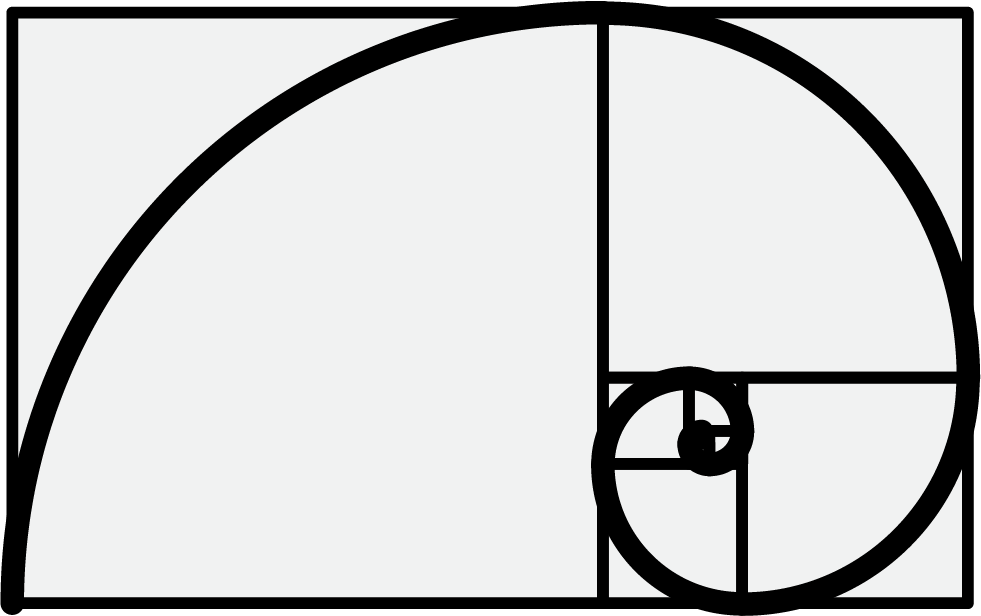
\includegraphics[height=0.75cm]{../../AAA_template_latex_settings/pwr-control_logo_doc.png}}
\lfoot{\href{http://www.pwr-control.com}{pwr-control.com}}
\cfoot{-\ \thepage\ -}
\rfoot{\textit{}}
\renewcommand{\headrulewidth}{0.4pt}
\renewcommand{\footrulewidth}{0.4pt}


\geometry{
	a4paper,
	top    = 2.5cm,
	bottom = 3.0cm,
	left   = 2.5cm,
	right  = 2.5cm
}

\hypersetup{
	colorlinks = true,
	urlcolor   = blue,
	linkcolor  = black,
	citecolor  = black
}

\pagenumbering{gobble}

\usetikzlibrary{decorations.pathreplacing,fit,shapes.geometric}
\usepackage[european,straightvoltages]{circuitikz}
\ctikzset{voltage dir=EF}

\newcommand{\ped}[1]{_{\mathrm{#1}}}
\newcommand{\code}[1]{\texttt{#1}}
\renewcommand{\tabularxcolumn}[1]{>{\raggedright\arraybackslash}p{#1}}
\setlength{\emergencystretch}{3em}

% ---------------- document metadata (read by the title page) ----------------
\newcommand{\DocCategory}{Technical Design Note}
\newcommand{\DocField}{Power Electronics and Control Systems}

\newcommand{\DocTitle}{%
	{\fontsize{20}{24}\selectfont\bfseries Three-phase dual active bridge (DAB3)} \\[16pt]
	{\fontsize{16}{20}\selectfont\bfseries \SI{1200}{\volt} / \SI{1200}{\volt}, \SI{250}{\kilo\watt}, \SI{10}{\kilo\hertz}: sizing, control, simulation model and runs}
}

\newcommand{\DocSubtitle}{%
	Isolated bidirectional DC/DC stage with two six-step bridges of SiC modules and three single-phase transformers in star-star, with the DC bias of the transformers and the first four runs of the Simscape bench.
}

\newcommand{\DocAuthor}{Davide Bagnara}
\newcommand{\DocRevision}{00}
\newcommand{\DocDate}{October 2026}

\newcommand{\DocAbstract}{%
	The three-phase dual active bridge (DAB3) transfers power between two DC links through two three-phase bridges driven with six-step voltages and three single-phase transformers in star-star with floating star points; the power is set by the phase displacement between the two bridges. This note documents the \SI{250}{\kilo\watt} DAB3 of the folder \code{analysis\_three\_phase\_dab} of \code{pwr-control/advanced-dcdc-converters}, between two batteries at about \SI{1200}{\volt}, with the transformers at \SI{10}{\kilo\hertz}. The sizing is derived step by step on a harmonic model of the converter (operating point, series inductance and phase shift, transformer and choice of the frequency, SiC modules and zero-voltage switching, DC links, loss budget), and the DAB3 is compared with the single-phase DAB at the same point. The current control, with its feed-forward, is designed on the LC of the DC side, and its sample rate is discussed for a control that runs at the transformer frequency or slower. A section is given to the DC bias of the transformers: where it comes from, what limits it, how to start the converter and how to update the phase shift without creating it, and how to measure and cancel it when the current is sampled no faster than the switching frequency. The second part describes the Simscape bench, built with the blocks of \code{pwr-control/library} and a parameter structure of its own, the changes made to the original model (which ran the transformers at \SI{2}{\kilo\hertz}), the numerical settings and their artefacts, and the first four runs: forward and reverse power at \SI{1}{pu}, light load, and voltage mismatch. The runs agree with the harmonic model within \SI{2}{\percent} on the currents and the switching currents and confirm the map of the soft-switching range.
}

\newcommand{\RevisionHistory}{%
	00 & October 2026 & First issue: sizing, control, DC bias of the transformers, simulation bench and runs 01 to 04. & \DocAuthor \\
}

\newcommand{\MetaLabelA}{Project Repository}
\newcommand{\MetaValueAUrl}{https://github.com/pwr-control/advanced-dcdc-converters.git}
\newcommand{\MetaValueALabel}{advanced-dcdc-converters.git}

\newcommand{\MetaLabelB}{Framework}
\newcommand{\MetaValueB}{MATLAB/Simulink/Simscape}

\begin{document}

% =============================================================
%  pwr-control LaTeX template - FRONTESPIZIO
%
%  Da richiamare come prima istruzione dopo \begin{document}:
%      % =============================================================
%  pwr-control LaTeX template - FRONTESPIZIO
%
%  Da richiamare come prima istruzione dopo \begin{document}:
%      % =============================================================
%  pwr-control LaTeX template - FRONTESPIZIO
%
%  Da richiamare come prima istruzione dopo \begin{document}:
%      \input{../../AAA_template_latex_settings/titlepage}
%
%  Il documento deve definire prima di \begin{document}:
%      \DocCategory   categoria del documento
%      \DocField      area tecnica
%      \DocTitle      titolo (una o due righe)
%      \DocSubtitle   sottotitolo
%      \DocAuthor     autore/i, separati da virgola
%      \DocRevision   numero di revisione corrente (es. 00)
%      \DocDate       data della revisione corrente
%      \DocAbstract   abstract
%      \RevisionHistory  righe della tabella di revisione, nel formato
%                        Rev. & Date & Description & Authors \\
%      \MetaLabelA \MetaValueAUrl \MetaValueALabel
%      \MetaLabelB \MetaValueB
% =============================================================

\providecommand{\DocCategory}{Technical Research Report}
\providecommand{\DocField}{Power Electronics and Control Systems}
\providecommand{\DocSubtitle}{}
\providecommand{\DocRevision}{00}
\providecommand{\DocAbstract}{}
\providecommand{\RevisionHistory}{%
	\DocRevision & \DocDate & First issue. & \DocAuthor \\
}

\titlepage

% ---- Intestazione centrata ----
\begin{center}
	{\Large\scshape \DocCategory}\\[8pt]
	{\large\scshape \DocField}
\end{center}

\vspace{30pt plus 4pt minus 14pt}
\noindent\rule{\linewidth}{0.8pt}

% ---- Titolo ----
\begin{center}
	\DocTitle
\end{center}

\vspace{4pt}
\noindent\rule{\linewidth}{2.2pt}

% ---- Sottotitolo ----
\begin{center}
	\begin{onehalfspace}
		{\large\itshape \DocSubtitle}
	\end{onehalfspace}
\end{center}

% ---- Authors / Revision / Date ----
\vspace{30pt plus 4pt minus 14pt}

\noindent
\begin{minipage}[t]{0.46\linewidth}
	\raggedright
	\textbf{Authors:}\\[2pt]
	\DocAuthor
\end{minipage}%
\hfill
\begin{minipage}[t]{0.22\linewidth}
	\centering
	\textbf{Revision:}\\[2pt]
	\DocRevision
\end{minipage}%
\hfill
\begin{minipage}[t]{0.30\linewidth}
	\raggedleft
	\textbf{Date:}\\[2pt]
	\DocDate
\end{minipage}

\vspace{10pt}
\noindent\rule{\linewidth}{0.8pt}

% ---- Abstract ----
\vspace{24pt plus 4pt minus 12pt}

\begin{center}
	\begin{minipage}{0.88\linewidth}
		\footnotesize
		\begin{onehalfspace}
			\textbf{Abstract:} \DocAbstract
		\end{onehalfspace}
	\end{minipage}
\end{center}

\vfill

% ---- Revision history ----
\begin{center}
	\begin{minipage}{0.96\linewidth}
		\centering
		{\footnotesize\scshape Revision history}\\[6pt]
		{\footnotesize
			\begin{tabular}{@{}cl>{\raggedright\arraybackslash}p{0.36\linewidth}>{\raggedright\arraybackslash}p{0.28\linewidth}@{}}
				\toprule
				\textbf{Rev.} & \textbf{Date} & \textbf{Description} & \textbf{Authors} \\
				\midrule
				\RevisionHistory
				\bottomrule
			\end{tabular}}
	\end{minipage}
\end{center}

\vspace{18pt plus 4pt minus 10pt}

% ---- Metadati in fondo ----
\noindent
\begin{tabular}{@{} r @{\quad} l @{}}
	\textsc{\MetaLabelA:} & {\href{\MetaValueAUrl}{\MetaValueALabel}} \\[3pt]
	\textsc{\MetaLabelB:} & {\MetaValueB}       \\[3pt]
\end{tabular}

% =============================================================
%  Fine frontespizio
% =============================================================
\newpage
\pagenumbering{arabic}
\setcounter{page}{1}

%
%  Il documento deve definire prima di \begin{document}:
%      \DocCategory   categoria del documento
%      \DocField      area tecnica
%      \DocTitle      titolo (una o due righe)
%      \DocSubtitle   sottotitolo
%      \DocAuthor     autore/i, separati da virgola
%      \DocRevision   numero di revisione corrente (es. 00)
%      \DocDate       data della revisione corrente
%      \DocAbstract   abstract
%      \RevisionHistory  righe della tabella di revisione, nel formato
%                        Rev. & Date & Description & Authors \\
%      \MetaLabelA \MetaValueAUrl \MetaValueALabel
%      \MetaLabelB \MetaValueB
% =============================================================

\providecommand{\DocCategory}{Technical Research Report}
\providecommand{\DocField}{Power Electronics and Control Systems}
\providecommand{\DocSubtitle}{}
\providecommand{\DocRevision}{00}
\providecommand{\DocAbstract}{}
\providecommand{\RevisionHistory}{%
	\DocRevision & \DocDate & First issue. & \DocAuthor \\
}

\titlepage

% ---- Intestazione centrata ----
\begin{center}
	{\Large\scshape \DocCategory}\\[8pt]
	{\large\scshape \DocField}
\end{center}

\vspace{30pt plus 4pt minus 14pt}
\noindent\rule{\linewidth}{0.8pt}

% ---- Titolo ----
\begin{center}
	\DocTitle
\end{center}

\vspace{4pt}
\noindent\rule{\linewidth}{2.2pt}

% ---- Sottotitolo ----
\begin{center}
	\begin{onehalfspace}
		{\large\itshape \DocSubtitle}
	\end{onehalfspace}
\end{center}

% ---- Authors / Revision / Date ----
\vspace{30pt plus 4pt minus 14pt}

\noindent
\begin{minipage}[t]{0.46\linewidth}
	\raggedright
	\textbf{Authors:}\\[2pt]
	\DocAuthor
\end{minipage}%
\hfill
\begin{minipage}[t]{0.22\linewidth}
	\centering
	\textbf{Revision:}\\[2pt]
	\DocRevision
\end{minipage}%
\hfill
\begin{minipage}[t]{0.30\linewidth}
	\raggedleft
	\textbf{Date:}\\[2pt]
	\DocDate
\end{minipage}

\vspace{10pt}
\noindent\rule{\linewidth}{0.8pt}

% ---- Abstract ----
\vspace{24pt plus 4pt minus 12pt}

\begin{center}
	\begin{minipage}{0.88\linewidth}
		\footnotesize
		\begin{onehalfspace}
			\textbf{Abstract:} \DocAbstract
		\end{onehalfspace}
	\end{minipage}
\end{center}

\vfill

% ---- Revision history ----
\begin{center}
	\begin{minipage}{0.96\linewidth}
		\centering
		{\footnotesize\scshape Revision history}\\[6pt]
		{\footnotesize
			\begin{tabular}{@{}cl>{\raggedright\arraybackslash}p{0.36\linewidth}>{\raggedright\arraybackslash}p{0.28\linewidth}@{}}
				\toprule
				\textbf{Rev.} & \textbf{Date} & \textbf{Description} & \textbf{Authors} \\
				\midrule
				\RevisionHistory
				\bottomrule
			\end{tabular}}
	\end{minipage}
\end{center}

\vspace{18pt plus 4pt minus 10pt}

% ---- Metadati in fondo ----
\noindent
\begin{tabular}{@{} r @{\quad} l @{}}
	\textsc{\MetaLabelA:} & {\href{\MetaValueAUrl}{\MetaValueALabel}} \\[3pt]
	\textsc{\MetaLabelB:} & {\MetaValueB}       \\[3pt]
\end{tabular}

% =============================================================
%  Fine frontespizio
% =============================================================
\newpage
\pagenumbering{arabic}
\setcounter{page}{1}

%
%  Il documento deve definire prima di \begin{document}:
%      \DocCategory   categoria del documento
%      \DocField      area tecnica
%      \DocTitle      titolo (una o due righe)
%      \DocSubtitle   sottotitolo
%      \DocAuthor     autore/i, separati da virgola
%      \DocRevision   numero di revisione corrente (es. 00)
%      \DocDate       data della revisione corrente
%      \DocAbstract   abstract
%      \RevisionHistory  righe della tabella di revisione, nel formato
%                        Rev. & Date & Description & Authors \\
%      \MetaLabelA \MetaValueAUrl \MetaValueALabel
%      \MetaLabelB \MetaValueB
% =============================================================

\providecommand{\DocCategory}{Technical Research Report}
\providecommand{\DocField}{Power Electronics and Control Systems}
\providecommand{\DocSubtitle}{}
\providecommand{\DocRevision}{00}
\providecommand{\DocAbstract}{}
\providecommand{\RevisionHistory}{%
	\DocRevision & \DocDate & First issue. & \DocAuthor \\
}

\titlepage

% ---- Intestazione centrata ----
\begin{center}
	{\Large\scshape \DocCategory}\\[8pt]
	{\large\scshape \DocField}
\end{center}

\vspace{30pt plus 4pt minus 14pt}
\noindent\rule{\linewidth}{0.8pt}

% ---- Titolo ----
\begin{center}
	\DocTitle
\end{center}

\vspace{4pt}
\noindent\rule{\linewidth}{2.2pt}

% ---- Sottotitolo ----
\begin{center}
	\begin{onehalfspace}
		{\large\itshape \DocSubtitle}
	\end{onehalfspace}
\end{center}

% ---- Authors / Revision / Date ----
\vspace{30pt plus 4pt minus 14pt}

\noindent
\begin{minipage}[t]{0.46\linewidth}
	\raggedright
	\textbf{Authors:}\\[2pt]
	\DocAuthor
\end{minipage}%
\hfill
\begin{minipage}[t]{0.22\linewidth}
	\centering
	\textbf{Revision:}\\[2pt]
	\DocRevision
\end{minipage}%
\hfill
\begin{minipage}[t]{0.30\linewidth}
	\raggedleft
	\textbf{Date:}\\[2pt]
	\DocDate
\end{minipage}

\vspace{10pt}
\noindent\rule{\linewidth}{0.8pt}

% ---- Abstract ----
\vspace{24pt plus 4pt minus 12pt}

\begin{center}
	\begin{minipage}{0.88\linewidth}
		\footnotesize
		\begin{onehalfspace}
			\textbf{Abstract:} \DocAbstract
		\end{onehalfspace}
	\end{minipage}
\end{center}

\vfill

% ---- Revision history ----
\begin{center}
	\begin{minipage}{0.96\linewidth}
		\centering
		{\footnotesize\scshape Revision history}\\[6pt]
		{\footnotesize
			\begin{tabular}{@{}cl>{\raggedright\arraybackslash}p{0.36\linewidth}>{\raggedright\arraybackslash}p{0.28\linewidth}@{}}
				\toprule
				\textbf{Rev.} & \textbf{Date} & \textbf{Description} & \textbf{Authors} \\
				\midrule
				\RevisionHistory
				\bottomrule
			\end{tabular}}
	\end{minipage}
\end{center}

\vspace{18pt plus 4pt minus 10pt}

% ---- Metadati in fondo ----
\noindent
\begin{tabular}{@{} r @{\quad} l @{}}
	\textsc{\MetaLabelA:} & {\href{\MetaValueAUrl}{\MetaValueALabel}} \\[3pt]
	\textsc{\MetaLabelB:} & {\MetaValueB}       \\[3pt]
\end{tabular}

% =============================================================
%  Fine frontespizio
% =============================================================
\newpage
\pagenumbering{arabic}
\setcounter{page}{1}


\tableofcontents
\listoffigures
\listoftables
\newpage

\begin{onehalfspace}

% =============================================================
\section*{Nomenclature}
\addcontentsline{toc}{section}{Nomenclature}
\label{sec:nomenclature}

\begingroup
\rowcolors{2}{tableShade}{white}
\begin{longtable}{@{} l p{0.72\linewidth} @{}}
	\toprule
	\textbf{Symbol} & \textbf{Meaning} \\
	\midrule
	\endfirsthead
	\toprule
	\textbf{Symbol} & \textbf{Meaning} \\
	\midrule
	\endhead
	\bottomrule
	\endfoot
	\bottomrule
	\endlastfoot
	$V\ped{1}$, $V\ped{2}$ & DC voltages of side 1 and side 2, \SI{1200}{\volt} nominal \\
	$n = n\ped{1}/n\ped{2}$ & turns ratio of the three transformers, $14:14$ \\
	$V\ped{2}' = n V\ped{2}$ & voltage of side 2 referred to side 1 \\
	$d = V\ped{2}'/V\ped{1}$ & voltage ratio \\
	$P$, $P\ped{nom}$ & power from side 1 to side 2; nominal power, \SI{250}{\kilo\watt} in both directions \\
	$f\ped{s}$, $\omega$, $T\ped{s}$ & transformer frequency, which is also the switching frequency of every device, \SI{10}{\kilo\hertz}; $\omega = 2\pi f\ped{s}$; $T\ped{s} = 1/f\ped{s}$ \\
	$f\ped{PWM}$ & clock of the library modulator, one step of the six-step pattern per period: $f\ped{PWM} = 6 f\ped{s} = \SI{60}{\kilo\hertz}$ \\
	$\theta = \omega t$ & angle within the period, $\theta = 0$ at the rising edge of leg a of bridge 1 \\
	$\varphi$ & phase displacement of bridge 2 after bridge 1; the power flows from side 1 to side 2 for $\varphi > 0$ \\
	$\varphi\ped{nom}$, $\varphi\ped{max}$ & phase shift at nominal power (\ang{30}); limit of the modulator (\ang{60}) \\
	$u$ & output of the current control, $u \in [-1, 1]$, $\varphi = u\,\varphi\ped{max}$ \\
	$L$ & series inductance of a phase, referred to side 1: $L = L\ped{d1} + L\ped{d2}'$ \\
	$L\ped{d1}$, $L\ped{d2}$ & leakage plus external inductance of the primary and of the secondary \\
	$L\ped{m}$, $R\ped{fe}$ & magnetizing inductance and core-loss resistance, primary side \\
	$R\ped{s1}$, $R\ped{s2}$ & resistance of winding, terminations and external inductor, primary and secondary \\
	$R\ped{1}$, $R\ped{2}$ & series resistance of a phase: $R\ped{s1}$ or $R\ped{s2}$ plus the on-resistance of the switch \\
	$u\ped{1x}$, $u\ped{2x}$ & phase-to-star-point voltages of bridge 1 and bridge 2, $x \in \{a, b, c\}$ \\
	$i\ped{1x}$, $i\ped{2x}$ & phase currents, out of leg $x$ of bridge 1 and into leg $x$ of bridge 2 \\
	$i\ped{m}$ & magnetizing current with the core-loss current, primary side \\
	$i\ped{dc1}$, $i\ped{dc2}$ & DC currents of the bridges: into bridge 1 from DC link 1, out of bridge 2 into DC link 2 \\
	$I\ped{dc1}$ & DC input current of side 1, the current of the DC choke where it enters the DC link (the controlled quantity) \\
	$i\ped{sw1}$, $i\ped{sw2}$ & switching currents of the two bridges, positive when they charge the leg capacitances in the direction of zero-voltage switching \\
	$C\ped{oss}$ & output capacitance of a switch \\
	$t\ped{d}$ & dead time, \SI{500}{\nano\second} \\
	$t\ped{c}$ & step of the Simscape local solver, \SI{100}{\nano\second} in the runs \\
	$\lambda$, $B$ & flux linkage of a winding and flux density of its core \\
	$N$, $A\ped{c}$ & turns and core area of a transformer \\
	$C\ped{dc}$, $L\ped{dc}$ & DC-link capacitor and DC choke of each side \\
	$k\ped{ff}$ & gain of the feed-forward of the current control \\
	$k\ped{p}$, $k\ped{i}$ & gains of the PI of the current control \\
	$h$ & harmonic order, $h = 6k \pm 1$ \\
	pu & per unit; the current base is $P\ped{nom}/V\ped{1} = \SI{208}{\ampere}$ \\
	ZVS & zero-voltage switching \\
	SoC & state of charge of a battery \\
	BE & Backward Euler integration method \\
\end{longtable}
\addtocounter{table}{-1}
%\rowcolors{1}{white}{white}
\endgroup
% =============================================================
\section{Introduction and scope}
\label{sec:intro}

The solid state transformer study of \cite{sst_doc} compared three isolated DC/DC stages at about \SI{250}{\kilo\watt} per phase: the three-phase dual active bridge of De Doncker, Divan and Kheraluwala \cite{dedoncker1991} (DAB3) at \SI{4}{\kilo\hertz} on three single-phase transformers of nanocrystalline cut cores, the single-phase DAB and the CLLC, the stage that the SST bench of today uses \cite{cllc_doc}. The study left the DAB3 to the repository \code{advanced-dcdc-converters} \cite{dcdc_repo}. This note is that continuation: it documents the folder \path{analysis_three_phase_dab} of the repository, turned into a \SI{250}{\kilo\watt} isolated bidirectional DC/DC stage between two batteries.

Figure~\ref{fig:converter} is the converter. Each side has a battery behind a DC choke and a DC-link capacitor. The two three-phase bridges of \SI{2}{\kilo\volt} SiC MOSFET half-bridge modules make six-step voltages at the transformer frequency $f\ped{s} = \SI{10}{\kilo\hertz}$. Three single-phase transformers, one per phase, are connected in star on both sides with the star points floating; their leakage, completed by an external inductor, is the series inductance that carries the power. The only control variable is the phase displacement $\varphi$ of bridge 2 after bridge 1, set by a loop on the DC input current of side 1.

\begin{figure}[H]
	\centering
	\begin{circuitikz}[scale=0.76, transform shape, font=\small, >=Latex,
		blk/.style={draw, thick, rounded corners=2pt, align=center, minimum height=1.1cm, fill=green!6},
		sumn/.style={draw, thick, circle, inner sep=1.5pt}]
		\ctikzset{bipoles/length=0.9cm}
		% side 1
		\draw (0,0) to[battery1, l=battery 1] (0,3);
		\draw (0,3) to[L, l=$L\ped{dc1}$] (1.7,3) to[short, i=$I\ped{dc1}$] (2.9,3);
		\draw (0,0) -- (3.4,0);
		\draw (2.9,3) -- (3.4,3);
		\draw (2.9,3) to[C, l_=$C\ped{dc1}$] (2.9,0);
		% bridge 1
		\draw[thick, fill=blue!6] (3.4,-0.4) rectangle (5.0,3.4);
		\node[align=center] at (4.2,1.5) {bridge 1\\six-step\\3 legs\\SiC};
		% phases and transformers
		\foreach \y/\p in {2.6/a, 1.5/b, 0.4/c} {
			\draw (5.0,\y) -- (5.7,\y) node[above, pos=0.5, font=\footnotesize] {\p};
			\draw (9.4,\y) -- (10.1,\y);
		}
		\draw[thick, fill=orange!12] (5.7,-0.4) rectangle (9.4,3.4);
		\node[align=center, font=\footnotesize] at (7.55,1.5) {3 single-phase\\transformers, $14:14$\\Y-Y, floating stars\\[2pt]$L\ped{d1} + L\ped{d2}' = \SI{28}{\micro\henry}$\\$L\ped{m} = \SI{1}{\milli\henry}$, gapped};
		% bridge 2
		\draw[thick, fill=blue!6] (10.1,-0.4) rectangle (11.7,3.4);
		\node[align=center] at (10.9,1.5) {bridge 2\\six-step\\3 legs\\lags by $\varphi$};
		% side 2
		\draw (11.7,3) -- (13.4,3); \draw (11.7,0) -- (16.4,0);
		\draw (12.4,3) to[C, l=$C\ped{dc2}$] (12.4,0);
		\draw (13.4,3) to[L, l=$L\ped{dc2}$] (15.1,3) -- (16.4,3);
		\draw (16.4,0) to[battery1, l_=battery 2] (16.4,3);
		% control
		\node[blk] (ref) at (0.9,-3.0) {bench\\$i\ped{ref}$};
		\node[blk] (rl) at (3.2,-3.0) {rate limiter\\\SI{20}{\pu\per\second}};
		\node[sumn] (s1) at (5.0,-3.0) {};
		\node[blk] (pi) at (6.6,-3.0) {PI\\$k\ped{p}$, $k\ped{i}$};
		\node[sumn] (s2) at (8.3,-3.0) {};
		\node[blk, fill=orange!10] (mod) at (10.9,-3.0) {modulator\\$\varphi = u\,\varphi\ped{max}$};
		\node[blk, minimum height=0.8cm] (ff) at (6.6,-4.4) {$k\ped{ff}$};
		\draw[->] (ref) -- (rl);
		\draw[->] (rl) -- (s1) node[pos=0.8, above, font=\scriptsize] {$+$};
		\draw[->] (s1) -- (pi);
		\draw[->] (pi) -- (s2) node[pos=0.8, above, font=\scriptsize] {$+$};
		\draw[->] (s2) -- (mod) node[midway, above, font=\footnotesize] {$u$};
		\draw[->] (4.3,-3.0) |- (ff.west);
		\draw[->] (ff.east) -| (s2.south) node[pos=0.92, right, font=\scriptsize] {$+$};
		\draw[->] (5.0,-1.95) node[above, font=\footnotesize] {$I\ped{dc1}$ (DC choke)} -- (s1.north) node[pos=0.8, right, font=\scriptsize] {$-$};
		\draw[->, thick] (mod.north) -- (10.9,-0.4);
		\draw[->, thick] ([xshift=-8mm]mod.north) |- (4.2,-1.1) -- (4.2,-0.4);
		\node[font=\footnotesize, anchor=south west] at (6.0,-1.1) {gates of both bridges};
		\draw[decorate, decoration={brace, amplitude=5pt}] (3.4,3.7) -- (11.7,3.7) node[midway, above=5pt] {DAB3 (\code{dab\_modA})};
	\end{circuitikz}
	\captionsetup{width=0.85\textwidth, font=small}
	\caption[The DAB3 and its control.]{The DAB3 between two batteries, as in the bench of Section~\ref{sec:model}: DC chokes and DC links on both sides, two six-step bridges, three single-phase transformers in star-star with floating star points. The current loop regulates the DC input current of side 1, $I\ped{dc1}$, with a PI and a feed-forward of the reference; the modulator turns its output $u$ into the phase displacement $\varphi$ of bridge 2 after bridge 1.}
	\label{fig:converter}
\end{figure}

The work behind this note had four steps, each documented here. First, the initialization of the model was rewritten around a parameter structure of its own, with the numbers of this converter in \path{private/dab3_param.m}, independent of the data of the library \cite{library_repo} while still using its blocks and Simscape components. Second, the original model was reviewed: it ran the transformers at \SI{2}{\kilo\hertz} without showing it, its modulator limit was beyond the maximum of the power, and its DC links, chokes and batteries came from the data of the single-phase DAB (Section~\ref{sec:changes}). Third, the converter was sized at \SI{1200}{\volt} / \SI{1200}{\volt} and \SI{10}{\kilo\hertz} on a harmonic model (Sections~\ref{sec:principle} to~\ref{sec:control}). Fourth, four runs of the Simscape bench were checked against the harmonic model (Section~\ref{sec:runs}).

\noindent\textbf{Working assumptions.} The DC voltages (\SI{1200}{\volt} on both sides; the batteries of the bench stay between about \SI{1180}{\volt} and \SI{1270}{\volt}), the turns ratio $1:1$ and the transformer frequency of \SI{10}{\kilo\hertz} are assumptions, to be confirmed with the specification. With other values the procedure is the same and the numbers of Section~\ref{sec:sizing} change. The control of the hardware is expected to run at \SI{10}{\kilo\hertz} at most, that is at most once per period of the transformers: Sections~\ref{sec:sampling} and~\ref{sec:dcbias} take this into account.

% =============================================================
\section{Operating principle}
\label{sec:principle}

\subsection{Six-step bridges and star-star transformers}
\label{sec:sixstep}

Each leg of a bridge is switched at \SI{50}{\percent} duty and the three legs are displaced by \ang{120}. With the star points floating, the phase-to-star-point voltage of each transformer takes the levels $\pm V/3$ and $\pm 2V/3$, each for a sixth of the period (Figure~\ref{fig:waveforms}), and contains only the harmonics $h = 6k \pm 1$:
\begin{equation}
	u\ped{1a}(\theta) = \frac{2 V\ped{1}}{\pi} \sum_{h = 1, 5, 7, 11, \ldots} \frac{\sin h\theta}{h}, \qquad
	u\ped{2a}'(\theta) = \frac{2 V\ped{2}'}{\pi} \sum_{h = 1, 5, 7, 11, \ldots} \frac{\sin h(\theta - \varphi)}{h},
	\label{eq:sixstep}
\end{equation}
with leg a of bridge 1 rising at $\theta = 0$ and legs b and c \ang{120} and \ang{240} later. The fundamental has the amplitude $2V/\pi$, \SI{764}{\volt} at \SI{1200}{\volt} (\SI{936}{\volt} line to line, rms); the triplen harmonics, which would drive a zero-sequence current, cannot appear with floating star points. Each switch turns on and off once per period: the switching frequency of every device is the transformer frequency.

\subsection{Power transfer}
\label{sec:power}

With the converter lossless and the magnetizing inductance neglected, the series inductance $L = L\ped{d1} + L\ped{d2}'$ of each phase carries the power \cite{dedoncker1991}
\begin{equation}
	P(\varphi) = \frac{V\ped{1} V\ped{2}'}{\omega L} \cdot
	\begin{cases}
		\varphi\left(\dfrac{2}{3} - \dfrac{\abs{\varphi}}{2\pi}\right), & \abs{\varphi} \le \dfrac{\pi}{3},\\[3mm]
		\sign(\varphi)\left(\abs{\varphi} - \dfrac{\varphi^2}{\pi} - \dfrac{\pi}{18}\right), & \dfrac{\pi}{3} \le \abs{\varphi} \le \dfrac{2\pi}{3},
	\end{cases}
	\label{eq:power}
\end{equation}
which grows up to $\abs{\varphi} = \pi/2$, where $P\ped{max} = \frac{7\pi}{36}\,V\ped{1} V\ped{2}'/(\omega L)$, and falls beyond it (Figure~\ref{fig:pphi}). The control drives the library modulator with $u \in [-1, 1]$ and the modulator applies $\varphi = u\,\varphi\ped{max}$. The original model had $\varphi\ped{max} = 2\pi/3$: the maximum of the power was inside the range of $u$, and the gain of the plant changed sign at $u = 0.75$. With $\varphi\ped{max} = \pi/3$ the power is monotonic in $u$ and reaches \SI{429}{\kilo\watt} ($1.7\,P\ped{nom}$) at nominal voltages and \SI{364}{\kilo\watt} ($1.45\,P\ped{nom}$) with $d = 0.85$.

\begin{figure}[H]
	\centering
	\begin{tikzpicture}
		\begin{axis}[
			width=0.82\linewidth, height=6.6cm,
			xlabel={$\varphi$ [\si{\degree}]}, ylabel={$P$ [\si{\kilo\watt}]},
			xmin=0, xmax=120, ymin=0, ymax=540, xtick={0,15,30,45,60,75,90,105,120},
			grid=major, grid style={gray!25},
			legend style={at={(0.5,0.03)}, anchor=south, font=\footnotesize, fill=white},
			tick label style={font=\footnotesize}, label style={font=\small}]
			\addplot[thick, blue!70!black] table[x=phi, y=P_d100] {figures/power_phi.dat};
			\addlegendentry{Eq.~\eqref{eq:power}, $d = 1$}
			\addplot[thick, red!70!black, dashed] table[x=phi, y=P_h100] {figures/power_phi.dat};
			\addlegendentry{harmonic model with $L\ped{m}$, $R\ped{fe}$, $R$, $d = 1$}
			\addplot[thick, orange!80!black] table[x=phi, y=P_d085] {figures/power_phi.dat};
			\addlegendentry{Eq.~\eqref{eq:power}, $d = 0.85$}
			\draw[dashed, gray] (axis cs:60,0) -- (axis cs:60,540);
			\node[font=\footnotesize, anchor=north east, fill=white, inner sep=1pt] at (axis cs:59,530) {$\varphi\ped{max} = \ang{60}$};
			\draw[dotted, gray] (axis cs:0,250) -- (axis cs:120,250);
			\addplot[only marks, mark=*, mark size=2pt, blue!70!black] coordinates {(30,250)};
			\node[font=\footnotesize, anchor=north west] at (axis cs:31,245) {\SI{250}{\kilo\watt} at \ang{30}};
		\end{axis}
	\end{tikzpicture}
	\captionsetup{width=0.85\textwidth, font=small}
	\caption[Power against the phase shift.]{Power against the phase shift at \SI{1200}{\volt}, $L = \SI{28}{\micro\henry}$, \SI{10}{\kilo\hertz} (\code{figures/power\_phi.dat}): Eq.~\eqref{eq:power} at $d = 1$ and $d = 0.85$, and the harmonic model of Section~\ref{sec:harmonic} with the magnetizing branch and the resistances (power delivered to side 2). The modulator limit $\varphi\ped{max} = \ang{60}$ keeps the control on the rising part of the curve.}
	\label{fig:pphi}
\end{figure}

\subsection{Harmonic model}
\label{sec:harmonic}

The sizing and the checks of the runs use a steady-state model by harmonic superposition: \path{private/dab3_harmonic_op.m} in the repository, and the same model in \path{py/three_phase_dab_figures.py} for the figures of this note. Per phase, the transformer is the T equivalent referred to side 1: $Z\ped{1h} = R\ped{1} + jh\omega L\ped{d1}$ on side 1, the magnetizing branch $Z\ped{mh} = jh\omega L\ped{m} \parallel R\ped{fe}$, and $Z\ped{2h} = R\ped{2}' + jh\omega L\ped{d2}'$ on side 2, where $R\ped{1}$ and $R\ped{2}$ include the on-resistance of the switches. For each harmonic of Eq.~\eqref{eq:sixstep}, with $U\ped{1h} = 2V\ped{1}/(h\pi)$ and $U\ped{2h} = 2V\ped{2}'/(h\pi)\,e^{-jh\varphi}$,
\begin{equation}
	E\ped{h} = \frac{U\ped{1h}/Z\ped{1h} + U\ped{2h}/Z\ped{2h}}{1/Z\ped{1h} + 1/Z\ped{mh} + 1/Z\ped{2h}}, \qquad
	I\ped{1h} = \frac{U\ped{1h} - E\ped{h}}{Z\ped{1h}}, \qquad
	J\ped{2h} = \frac{E\ped{h} - U\ped{2h}}{Z\ped{2h}},
	\label{eq:harmonic}
\end{equation}
and the currents of phase a are $i\ped{1a}(\theta) = \sum_h \Im\{I\ped{1h} e^{jh\theta}\}$ and $i\ped{2a}(\theta) = n \sum_h \Im\{J\ped{2h} e^{jh\theta}\}$, the other phases \ang{120} and \ang{240} later. The quantities of the sizing follow from the phasors:
\begin{equation}
	P\ped{1} = \frac{3}{2}\sum_h \Re\{U\ped{1h} I\ped{1h}^*\}, \qquad
	\begin{aligned}
		i\ped{sw1} &= -i\ped{1a}(0) = -\sum_h \Im\{I\ped{1h}\},\\
		i\ped{sw2} &= i\ped{2a}(\varphi) = n\sum_h \Im\{J\ped{2h}\, e^{jh\varphi}\}.
	\end{aligned}
	\label{eq:isw}
\end{equation}
$i\ped{sw1}$ is the current that leg a of bridge 1 commutates at its rising edge, positive when it flows into the leg and charges the node upwards as ZVS requires; $i\ped{sw2}$ is the same for bridge 2, whose current is counted into the leg. The falling edges see the same currents with the opposite sign, by half-wave symmetry. In the lossless case the model agrees with Eq.~\eqref{eq:power} within \SI{0.05}{\percent}. With the magnetizing branch and the resistances it gives the currents, the switching currents, the magnetizing current and the ripple of the DC side used in the following sections, and each run of Section~\ref{sec:runs} is compared with it at the voltages and the phase shift measured in the run.

\subsection{Waveforms at the nominal point}
\label{sec:waveforms}

Figure~\ref{fig:waveforms} shows one period at \SI{1200}{\volt} / \SI{1200}{\volt} and $\varphi = \ang{30}$ with the numbers of Section~\ref{sec:sizing}. The phase currents are \SI{161}{\ampere} rms and \SI{240}{\ampere} peak. At its rising edge each leg of bridge 1 commutates \SI{124}{\ampere} flowing into the leg, each leg of bridge 2 \SI{125}{\ampere} flowing from the transformer into the leg: both bridges switch with ZVS (Section~\ref{sec:semi}). The magnetizing current follows the flux of the core, \SI{11.7}{\ampere} peak. The DC current of each bridge is the sum of the currents of the legs whose upper switch is on: it has the six-pulse shape at $6 f\ped{s} = \SI{60}{\kilo\hertz}$, between \SI{115}{\ampere} and \SI{240}{\ampere} around its mean of \SI{207}{\ampere}, that is \SI{40}{\ampere} rms of ripple for the DC-link capacitors.

\begin{figure}[H]
	\centering
	\begin{tikzpicture}
		\begin{axis}[
			width=0.88\linewidth, height=4.4cm,
			ylabel={[\si{\volt}]}, xmin=0, xmax=360, ymin=-950, ymax=950, xtick={0,60,...,360},
			xticklabels={}, grid=major, grid style={gray!25},
			legend columns=2, legend pos=north east, legend style={font=\footnotesize, fill=white},
			tick label style={font=\footnotesize}, label style={font=\small}]
			\addplot[thick, blue!70!black] table[x=theta, y=v1a] {figures/waveforms_nominal.dat};
			\addlegendentry{$u\ped{1a}$}
			\addplot[thick, red!70!black, dashed] table[x=theta, y=v2a] {figures/waveforms_nominal.dat};
			\addlegendentry{$u\ped{2a}$}
		\end{axis}
	\end{tikzpicture}

	\begin{tikzpicture}
		\begin{axis}[
			width=0.88\linewidth, height=4.6cm,
			ylabel={[\si{\ampere}]}, xmin=0, xmax=360, ymin=-260, ymax=260, xtick={0,60,...,360},
			xticklabels={}, grid=major, grid style={gray!25},
			legend columns=3, legend pos=north east, legend style={font=\footnotesize, fill=white},
			tick label style={font=\footnotesize}, label style={font=\small}]
			\addplot[thick, blue!70!black] table[x=theta, y=i1a] {figures/waveforms_nominal.dat};
			\addlegendentry{$i\ped{1a}$}
			\addplot[thick, red!70!black, dashed] table[x=theta, y=i2a] {figures/waveforms_nominal.dat};
			\addlegendentry{$i\ped{2a}$}
			\addplot[thick, orange!80!black] table[x=theta, y expr=10*\thisrow{im}] {figures/waveforms_nominal.dat};
			\addlegendentry{$10\,i\ped{m}$}
		\end{axis}
	\end{tikzpicture}

	\begin{tikzpicture}
		\begin{axis}[
			width=0.88\linewidth, height=4.4cm,
			xlabel={$\theta$ [\si{\degree}]}, ylabel={[\si{\ampere}]}, xmin=0, xmax=360, ymin=0, ymax=300, xtick={0,60,...,360},
			grid=major, grid style={gray!25},
			legend columns=2, legend pos=south east, legend style={font=\footnotesize, fill=white},
			tick label style={font=\footnotesize}, label style={font=\small}]
			\addplot[thick, blue!70!black] table[x=theta, y=idc1] {figures/waveforms_nominal.dat};
			\addlegendentry{$i\ped{dc1}$}
			\addplot[thick, red!70!black, dashed] table[x=theta, y=idc2] {figures/waveforms_nominal.dat};
			\addlegendentry{$i\ped{dc2}$}
		\end{axis}
	\end{tikzpicture}
	\captionsetup{width=0.85\textwidth, font=small}
	\caption[Waveforms at the nominal point.]{Steady state at \SI{1200}{\volt} / \SI{1200}{\volt}, $\varphi = \ang{30}$, from the harmonic model (\code{figures/waveforms\_nominal.dat}): phase-to-star-point voltages of the two bridges (top), phase currents of phase a on both sides and magnetizing current, scaled by 10 (middle), DC currents of the two bridges (bottom).}
	\label{fig:waveforms}
\end{figure}

\subsection{Why three phases}
\label{sec:why3ph}

Table~\ref{tab:compare1ph} compares the DAB3 with a single-phase DAB \cite{krismer2010, zhao2014} at the same point, both lossless and with the magnetizing inductance neglected (\path{py/three_phase_dab_figures.py}). For the same power and phase shift the DAB3 needs less series inductance per phase, its phase current is two thirds of the current of the single-phase converter, it turns off less than half the current at each commutation, and the ripple of its DC current is a third in amplitude at three times the frequency, so that with the same \SI{500}{\micro\farad} the voltage ripple of the DC link is six times smaller. The price is the number of switches, 12 against 8, and of magnetic components, three transformers with a third of the power each. With the same device in every position the conduction losses are \SI{30}{\percent} lower and the sum of the turned-off currents \SI{29}{\percent} lower; with the same total silicon area the conduction losses are about the same, and the advantage stays in the switching losses, in the DC links and in the volt-seconds per transformer. The 2025 comparison of \cite{sst_doc} found the single-phase DAB more efficient, but at different operating points (the single-phase DAB at \SI{12}{\kilo\hertz}, the DAB3 at \SI{4}{\kilo\hertz}, with different transformers), and it left the residual DC current of the single-phase transformer as an open question; Section~\ref{sec:dcbias} treats that question for the DAB3.

\begin{table}[H]
	\centering
	\captionsetup{width=0.9\textwidth, font=small}
	\caption[DAB3 and single-phase DAB at the same point.]{DAB3 and single-phase DAB at \SI{250}{\kilo\watt}, \SI{1200}{\volt} / \SI{1200}{\volt}, \SI{10}{\kilo\hertz}, $\varphi = \ang{30}$, lossless, $L\ped{m}$ infinite (\path{py/three_phase_dab_figures.py}).}
	\label{tab:compare1ph}
	\rowcolors{2}{tableShade}{white}
	\small
	\begin{tabularx}{0.97\textwidth}{@{} X >{\raggedright\arraybackslash}p{0.27\textwidth} >{\raggedright\arraybackslash}p{0.27\textwidth} @{}}
		\toprule
		\textbf{Quantity} & \textbf{DAB3} & \textbf{Single-phase DAB} \\
		\midrule
		Series inductance & \SI{28.0}{\micro\henry} per phase & \SI{40.0}{\micro\henry} \\
		Current of a winding & \SI{161}{\ampere} rms, \SI{238}{\ampere} peak & \SI{236}{\ampere} rms, \SI{250}{\ampere} peak \\
		Current at the commutations & \SI{119}{\ampere} & \SI{250}{\ampere} \\
		Switches; conduction with \SI{1.04}{\milli\ohm} each & 12; \SI{162}{\watt} & 8; \SI{231}{\watt} \\
		Sum of the turned-off currents per period & \SI{1428}{\ampere} ($12 \times \SI{119}{\ampere}$) & \SI{2000}{\ampere} ($8 \times \SI{250}{\ampere}$) \\
		Ripple current of the DC link & \SI{38.5}{\ampere} rms at \SI{60}{\kilo\hertz} & \SI{110.5}{\ampere} rms at \SI{20}{\kilo\hertz} \\
		Voltage ripple with \SI{500}{\micro\farad} & \SI{0.56}{\volt} peak to peak & \SI{3.5}{\volt} peak to peak \\
		Transformers & 3, \SI{13.3}{\milli\volt\second} each, \SI{274}{\kilo\volt\ampere} of windings per side & 1, \SI{30.0}{\milli\volt\second}, \SI{283}{\kilo\volt\ampere} \\
		\bottomrule
	\end{tabularx}
	\rowcolors{1}{white}{white}
\end{table}

% =============================================================
\section{Sizing of the \SI{250}{\kilo\watt} stage}
\label{sec:sizing}

\subsection{Operating point}
\label{sec:op}

Table~\ref{tab:op} is the operating point. Both DC voltages are \SI{1200}{\volt}, the voltage of the \SI{690}{\volt} application case of the library data used by the original model, so the transformers are $1:1$ and the same SiC module is used on both bridges. The base current of the control is $P\ped{nom}/V\ped{1} = \SI{208}{\ampere}$.

\begin{table}[H]
	\centering
	\captionsetup{width=0.9\textwidth, font=small}
	\caption{Operating point of the DAB3.}
	\label{tab:op}
	\rowcolors{2}{tableShade}{white}
	\small
	\begin{tabularx}{0.97\textwidth}{@{} >{\raggedright\arraybackslash}p{0.3\textwidth} >{\raggedright\arraybackslash}p{0.25\textwidth} X @{}}
		\toprule
		\textbf{Quantity} & \textbf{Value} & \textbf{Note} \\
		\midrule
		DC voltages $V\ped{1}$, $V\ped{2}$ & \SI{1200}{\volt} / \SI{1200}{\volt} & assumption; batteries of the bench \SI{1248}{\volt} at SoC 0.85 \\
		Turns ratio & 1 ($14:14$) & three single-phase transformers, Y-Y, floating star points \\
		Nominal power & \SI{250}{\kilo\watt} & both directions \\
		DC current & \SI{208}{\ampere} & base of the current loop \\
		Transformer frequency $f\ped{s}$ & \SI{10}{\kilo\hertz} & switching frequency of every device \\
		Clock of the modulator $f\ped{PWM}$ & \SI{60}{\kilo\hertz} $= 6 f\ped{s}$ & one step of the six-step pattern per period of the clock \\
		Series inductance $L$ & \SI{28}{\micro\henry} per phase & \SI{14}{\micro\henry} + \SI{14}{\micro\henry}, leakage and external inductor \\
		Phase shift at \SI{250}{\kilo\watt} & \ang{30} & Eq.~\eqref{eq:power} \\
		Limit of the modulator $\varphi\ped{max}$ & \ang{60} & \SI{429}{\kilo\watt} at $d = 1$, \SI{364}{\kilo\watt} at $d = 0.85$ \\
		Devices & \path{danfoss_SKM1700MB20R4S2I4} & \SI{2}{\kilo\volt} SiC half-bridge modules of the library datasets, \SI{1.04}{\milli\ohm}, $C\ped{oss} = \SI{3.28}{\nano\farad}$ \\
		Dead time $t\ped{d}$ & \SI{500}{\nano\second} & to be confirmed; not applied by the library modulator \\
		Current control & PI and feed-forward on $I\ped{dc1}$ & \SI{18}{\hertz} of bandwidth, Section~\ref{sec:control} \\
		\bottomrule
	\end{tabularx}
	\rowcolors{1}{white}{white}
\end{table}

\subsection{Series inductance and phase shift}
\label{sec:inductance}

The phase shift chosen for the nominal point sets the series inductance through Eq.~\eqref{eq:power}:
\begin{equation}
	L = \frac{V\ped{1} V\ped{2}'}{\omega P\ped{nom}}\,\varphi\ped{nom}\left(\frac{2}{3} - \frac{\varphi\ped{nom}}{2\pi}\right) = \SI{28.0}{\micro\henry} \quad (\varphi\ped{nom} = \ang{30}).
	\label{eq:L}
\end{equation}
Table~\ref{tab:phinom} shows the trade-off at \SI{10}{\kilo\hertz}. The rms current changes little with $\varphi\ped{nom}$. A small $\varphi\ped{nom}$ gives a large power gain $\mathrm{d}P/\mathrm{d}\varphi$, which makes the converter sensitive to the timing of the gates and to the resolution of the phase shift; a large one leaves less margin for the voltage range and for the transients. \ang{30} is the middle choice: \SI{28}{\micro\henry} per phase, $P\ped{max} = 2 P\ped{nom}$ at \ang{90} and $1.7 P\ped{nom}$ at $\varphi\ped{max}$. The library class \code{hw\_dab\_three\_phase\_setup} derives its own series inductance from the PWM frequency with the single-phase expression $V\ped{1}^2/(4 f\ped{PWM} P)$, \SI{24}{\micro\henry} with the inputs of this converter; \code{init\_model.m} writes the \SI{14}{\micro\henry} + \SI{14}{\micro\henry} of the sizing over it. The leakage of the transformers is estimated at about \SI{12}{\micro\henry} in total (Section~\ref{sec:transformer}); the rest is an external or integrated inductor.

\begin{table}[H]
	\centering
	\captionsetup{width=0.9\textwidth, font=small}
	\caption[Series inductance against the nominal phase shift.]{Series inductance against the nominal phase shift, \SI{250}{\kilo\watt}, \SI{1200}{\volt} / \SI{1200}{\volt}, \SI{10}{\kilo\hertz}; currents from the harmonic model with $L\ped{m} = \SI{1}{\milli\henry}$.}
	\label{tab:phinom}
	\rowcolors{2}{tableShade}{white}
	\small
	\begin{tabularx}{0.9\textwidth}{@{} l r X r X @{}}
		\toprule
		$\varphi\ped{nom}$ & $L$ per phase & Phase current, rms / peak & $i\ped{sw}$ & $P\ped{max}$ at $d = 1$ / $d = 0.85$ \\
		\midrule
		\ang{20} & \SI{19.6}{\micro\henry} & \SI{156}{\ampere} / \SI{229}{\ampere} & \SI{119}{\ampere} & \SI{716}{\kilo\watt} / \SI{609}{\kilo\watt} \\
		\ang{25} & \SI{23.9}{\micro\henry} & \SI{159}{\ampere} / \SI{234}{\ampere} & \SI{122}{\ampere} & \SI{586}{\kilo\watt} / \SI{498}{\kilo\watt} \\
		\textbf{\ang{30}} & \textbf{\SI{28.0}{\micro\henry}} & \textbf{\SI{161}{\ampere} / \SI{240}{\ampere}} & \textbf{\SI{124}{\ampere}} & \textbf{\SI{500}{\kilo\watt} / \SI{425}{\kilo\watt}} \\
		\ang{35} & \SI{31.9}{\micro\henry} & \SI{164}{\ampere} / \SI{245}{\ampere} & \SI{127}{\ampere} & \SI{439}{\kilo\watt} / \SI{373}{\kilo\watt} \\
		\ang{40} & \SI{35.6}{\micro\henry} & \SI{167}{\ampere} / \SI{251}{\ampere} & \SI{130}{\ampere} & \SI{394}{\kilo\watt} / \SI{335}{\kilo\watt} \\
		\bottomrule
	\end{tabularx}
	\rowcolors{1}{white}{white}
\end{table}

\subsection{Transformer}
\label{sec:transformer}

Each phase has its own single-phase transformer on the core set of the 2025 study \cite{sst_doc}: three AM-NC-320C nanocrystalline cut cores in parallel, $A\ped{c} = \SI{47}{\square\centi\metre}$, \SI{26.35}{\kilogram}. The phase-to-star voltage of the six-step pattern has the peak flux linkage
\begin{equation}
	\lambda\ped{pk} = \frac{V\ped{1}}{9 f\ped{s}} = \SI{13.3}{\milli\volt\second},
	\label{eq:lambda}
\end{equation}
half of the integral of $V/3$, $2V/3$, $V/3$ over three sixths of the period; at full load the drop on $L\ped{d1}$ lowers it to \SI{11.6}{\milli\volt\second}. With 14 turns the peak flux density is \SI{0.20}{\tesla} at no load and \SI{0.18}{\tesla} at full load (Table~\ref{tab:transformer}).

The magnetizing inductance is a choice. The gapped core with $L\ped{m} = \SI{1}{\milli\henry}$ costs a magnetizing current of about \SI{12}{\ampere} peak, which adds to the switching currents and keeps both bridges in ZVS down to \SI{9}{\percent} of the load at $d = 1$ (Section~\ref{sec:semi}); it also limits the flux offset that a DC current produces (Section~\ref{sec:dcbias}). With the relative permeability of 5000 of the cut cores \cite{sst_doc} and no gap, $L\ped{m}$ would be about \SI{8}{\milli\henry}: the ZVS limit at $d = 1$ would move from \SI{9}{\percent} to about \SI{15}{\percent} of the load, and the core would saturate with less than \SI{10}{\ampere} of DC.

\begin{table}[H]
	\centering
	\captionsetup{width=0.9\textwidth, font=small}
	\caption{Transformers, one per phase (values marked TBC to be confirmed with the design of the windings).}
	\label{tab:transformer}
	\rowcolors{2}{tableShade}{white}
	\small
	\begin{tabularx}{0.97\textwidth}{@{} >{\raggedright\arraybackslash}p{0.26\textwidth} >{\raggedright\arraybackslash}p{0.3\textwidth} X @{}}
		\toprule
		\textbf{Quantity} & \textbf{Value} & \textbf{Note} \\
		\midrule
		Core & 3 $\times$ AM-NC-320C, nanocrystalline cut cores & $A\ped{c} = \SI{47}{\square\centi\metre}$, \SI{26.35}{\kilogram}, the set of \cite{sst_doc} \\
		Peak flux linkage & \SI{13.3}{\milli\volt\second} & Eq.~\eqref{eq:lambda}; \SI{11.6}{\milli\volt\second} at full load \\
		Turns & $14:14$ & \SI{0.20}{\tesla} peak at no load, \SI{0.18}{\tesla} at full load \\
		Magnetizing inductance & \SI{1}{\milli\henry}, gapped & $i\ped{m}$ \SIrange{12}{13}{\ampere} peak; $\mu\ped{r,eff} = 622$ with $l\ped{e} = \SI{0.72}{\metre}$ (TBC) \\
		Core losses & about \SI{107}{\watt} & $R\ped{fe} = \SI{3}{\kilo\ohm}$; \SI{16}{\watt\per\kilogram} at \SI{4}{\kilo\hertz} and \SI{0.8}{\tesla} \cite{sst_doc}, scaled with $f^{1.5}B^2$ \\
		Windings, terminations, external inductor & $R\ped{s1} = R\ped{s2} = \SI{1.3}{\milli\ohm}$ (TBC) & \SI{68}{\watt} per transformer at \SI{161}{\ampere} rms \\
		Leakage & about \SI{12}{\micro\henry} in total & with \SI{10}{\milli\metre} between the windings; the rest of the \SI{28}{\micro\henry} is external \\
		\bottomrule
	\end{tabularx}
	\rowcolors{1}{white}{white}
\end{table}

\noindent\textbf{Choice of the frequency.} The transformer frequency is the main choice of the design. Table~\ref{tab:freq} compares four frequencies at the nominal point with the same core set, the turns set for $B \le \SI{0.35}{\tesla}$, the same devices, $L$ scaled for \ang{30} at \SI{250}{\kilo\watt}, and $L\ped{m}$ scaled to keep the same magnetizing current; the turn-off losses are the upper bound of Section~\ref{sec:losses}. The losses about double with each doubling of the frequency, driven by the turn-off and the core terms, while the transformer at \SI{2}{\kilo\hertz} needs 41 turns for five times the volt-seconds of \SI{10}{\kilo\hertz}. \SI{10}{\kilo\hertz} keeps the losses near \SI{1}{\percent} and the magnetics compact; \SI{5}{\kilo\hertz} is the conservative alternative. At \SI{10}{\kilo\hertz} the final design uses 14 turns instead of the 9 of the comparison, which lowers the flux density to \SI{0.20}{\tesla} and the core losses from \SI{776}{\watt} to \SI{320}{\watt}. The original model ran at \SI{2}{\kilo\hertz} without showing it: its PWM frequency was \SI{12}{\kilo\hertz} and the library modulator makes the six-step pattern at $f\ped{PWM}/6$.

\begin{table}[H]
	\centering
	\captionsetup{width=0.9\textwidth, font=small}
	\caption[Losses against the transformer frequency.]{Losses at \SI{250}{\kilo\watt} against the transformer frequency: same core set with the turns for $B \le \SI{0.35}{\tesla}$, same devices, \ang{30} at the nominal point. Losses in watts; the total includes the body diodes in the dead time (5 to \SI{52}{\watt}).}
	\label{tab:freq}
	\rowcolors{2}{tableShade}{white}
	\small
	\begin{tabularx}{0.97\textwidth}{@{} X r r r r r r r r @{}}
		\toprule
		$f\ped{s}$ & $L$ & $N$ & $B$ & Conduction & Turn-off & Windings & Cores & \textbf{Total} \\
		\midrule
		\SI{2}{\kilo\hertz} & \SI{140}{\micro\henry} & 41 & \SI{0.35}{\tesla} & 162 & 299 & 195 & 84 & \textbf{\SI{0.74}{\kilo\watt}} \\
		\SI{5}{\kilo\hertz} & \SI{56}{\micro\henry} & 17 & \SI{0.33}{\tesla} & 162 & 746 & 195 & 308 & \textbf{\SI{1.42}{\kilo\watt}} \\
		\SI{10}{\kilo\hertz} & \SI{28}{\micro\henry} & 9 & \SI{0.32}{\tesla} & 162 & 1493 & 195 & 776 & \textbf{\SI{2.65}{\kilo\watt}} \\
		\SI{20}{\kilo\hertz} & \SI{14}{\micro\henry} & 5 & \SI{0.28}{\tesla} & 162 & 2985 & 195 & 1778 & \textbf{\SI{5.17}{\kilo\watt}} \\
		\bottomrule
	\end{tabularx}
	\rowcolors{1}{white}{white}
\end{table}

\subsection{Semiconductors and zero-voltage switching}
\label{sec:semi}

Both bridges use the \SI{2}{\kilo\volt} SiC half-bridge module of the original model, the dataset \code{danfoss\_SKM1700MB20R4S2I4} of the library: \SI{1.04}{\milli\ohm}, $C\ped{oss} = \SI{3.28}{\nano\farad}$, $E\ped{on}$ and $E\ped{off}$ of \SI{77}{\milli\joule} and \SI{108}{\milli\joule} at \SI{1300}{\volt} and \SI{1000}{\ampere}. The module is oversized for \SI{161}{\ampere} rms (\SI{162}{\watt} of conduction for the 12 switches): a module of the \SIrange{300}{600}{\ampere} class would do, with a smaller $C\ped{oss}$ and a wider ZVS range.

At each commutation the current of the phase charges one $C\ped{oss}$ of the leg and discharges the other. The transition is complete within the dead time when
\begin{equation}
	i\ped{sw} \ge \frac{2 C\ped{oss} V}{t\ped{d}} = \SI{15.7}{\ampere} \qquad (V = \SI{1200}{\volt},\ t\ped{d} = \SI{500}{\nano\second}),
	\label{eq:zvs}
\end{equation}
and it lasts $2 C\ped{oss} V/i\ped{sw}$. At the nominal point $i\ped{sw} = \SI{124}{\ampere}$ on both bridges and the transition takes \SI{63}{\nano\second}. With $d \ne 1$ the bridge of the lower voltage loses its switching current at light load: Figure~\ref{fig:zvsmap} and Table~\ref{tab:zvs} give, from the harmonic model, the lowest load above which each bridge has the current of Eq.~\eqref{eq:zvs}. At $d = 1$ the magnetizing current keeps both bridges in ZVS down to \SI{9}{\percent} of the load; a mismatch of \SI{5}{\percent} moves the limit to about \SI{30}{\percent}, a mismatch of \SI{15}{\percent} to 59 or \SI{72}{\percent}. This is the known limit of the DAB3 with six-step voltages and phase shift only \cite{dedoncker1991}. If the batteries can differ by more than about \SI{5}{\percent}, the options are a DC link that follows the battery (a front-end stage), a lower $L\ped{m}$, or a modulation with a third degree of freedom, such as pulse width or asymmetric pulses.

\begin{figure}[H]
	\centering
	\begin{tikzpicture}
		\begin{axis}[
			width=0.8\linewidth, height=6.6cm,
			xlabel={$d = V\ped{2}'/V\ped{1}$}, ylabel={load [\si{\percent}]},
			xmin=0.8, xmax=1.2, ymin=0, ymax=100,
			grid=major, grid style={gray!25},
			legend pos=north east, legend style={font=\footnotesize, fill=white},
			tick label style={font=\footnotesize}, label style={font=\small}]
			\addplot[thick, blue!70!black] table[x=d, y=x1] {figures/zvs_map.dat};
			\addlegendentry{bridge 1}
			\addplot[thick, red!70!black, dashed] table[x=d, y=x2] {figures/zvs_map.dat};
			\addlegendentry{bridge 2}
			\addplot[only marks, mark=*, mark size=2.2pt, black] coordinates {(1.049,100) (1.005,10.3) (0.962,25.7)};
			\addlegendentry{runs 01, 03, 04}
			\node[font=\footnotesize, anchor=north east] at (axis cs:1.045,99) {01};
			\node[font=\footnotesize, anchor=south west] at (axis cs:1.008,10.5) {03};
			\node[font=\footnotesize, anchor=south east] at (axis cs:0.958,26) {04};
			\node[font=\footnotesize, align=center] at (axis cs:0.88,15) {bridge 2\\without ZVS};
			\node[font=\footnotesize, align=center] at (axis cs:1.13,15) {bridge 1\\without ZVS};
		\end{axis}
	\end{tikzpicture}
	\captionsetup{width=0.85\textwidth, font=small}
	\caption[ZVS boundaries against load and voltage ratio.]{Lowest load at which each bridge commutates the current of Eq.~\eqref{eq:zvs} within the dead time of \SI{500}{\nano\second}, forward power, $V\ped{1} = \SI{1200}{\volt}$, harmonic model with $L\ped{m} = \SI{1}{\milli\henry}$ (\code{figures/zvs\_map.dat}); ZVS above the lines. The points are the forward runs of Section~\ref{sec:runs} at their measured $d$ and load. In reverse power the roles of the bridges are exchanged and $d$ is replaced by $1/d$.}
	\label{fig:zvsmap}
\end{figure}

\begin{table}[H]
	\centering
	\captionsetup{width=0.9\textwidth, font=small}
	\caption{Lowest load with ZVS of each bridge against the voltage ratio (Figure~\ref{fig:zvsmap}).}
	\label{tab:zvs}
	\rowcolors{2}{tableShade}{white}
	\small
	\begin{tabular}{@{} l r r r r r r r @{}}
		\toprule
		$d$ & 0.85 & 0.90 & 0.95 & 1.00 & 1.05 & 1.10 & 1.15 \\
		\midrule
		Bridge 1 & 0 & 0 & 0 & \SI{9}{\percent} & \SI{31}{\percent} & \SI{52}{\percent} & \SI{72}{\percent} \\
		Bridge 2 & \SI{59}{\percent} & \SI{45}{\percent} & \SI{29}{\percent} & \SI{9}{\percent} & 0 & 0 & 0 \\
		\bottomrule
	\end{tabular}
	\rowcolors{1}{white}{white}
\end{table}

\noindent\textbf{The model does not simulate the transitions.} The library modulator does not apply its dead-time parameter and the bridges have no $C\ped{oss}$: the legs switch at once. The runs give the switching currents, with their sign and value at the edges, and the transition times are computed from them with Eq.~\eqref{eq:zvs}.

\subsection{DC links and chokes}
\label{sec:dclinks}

The DC current of each bridge has the six-pulse ripple of Figure~\ref{fig:waveforms}, \SI{40}{\ampere} rms at \SI{60}{\kilo\hertz} at full load, which gives \SI{0.6}{\volt} peak to peak on \SI{500}{\micro\farad}: the DC links are film banks sized on the ripple current rather than on the voltage ripple. Between the batteries and the DC links there are chokes of \SI{250}{\micro\henry} and \SI{2}{\milli\ohm}. With the DC link they resonate at \SI{450}{\hertz}, damped by the internal resistance of the battery (\SI{72}{\milli\ohm} with the settings of the bench), and this resonance limits the bandwidth of the current loop (Section~\ref{sec:control}). The DC links and the batteries start at the open-circuit voltage of the batteries. The values of the DC side are those of the bench and are still to be confirmed.

\subsection{Loss budget}
\label{sec:losses}

Table~\ref{tab:losses} is the estimate at \SI{250}{\kilo\watt}. The turn-off term scales the $E\ped{off}$ of the dataset linearly with voltage and current to \SI{124}{\ampere}. It is an upper bound: with ZVS the $C\ped{oss}$ acts as a snubber and the turn-off energy is a fraction of the hard-switching one. The soft turn-off energy of the module at \SI{1200}{\volt} and \SIrange{100}{150}{\ampere} is the missing number: with it the efficiency is between \SI{99.0}{\percent} and \SI{99.6}{\percent}.

\begin{table}[H]
	\centering
	\captionsetup{width=0.9\textwidth, font=small}
	\caption{Loss budget at \SI{250}{\kilo\watt} (sizing estimate).}
	\label{tab:losses}
	\rowcolors{2}{tableShade}{white}
	\small
	\begin{tabularx}{0.9\textwidth}{@{} l r X @{}}
		\toprule
		\textbf{Item} & \textbf{Loss} & \textbf{Basis} \\
		\midrule
		Conduction, 12 switches & \SI{162}{\watt} & \SI{1.04}{\milli\ohm}, \SI{161}{\ampere} rms per leg \\
		Turn-off, 12 switches & $\le \SI{1490}{\watt}$ & $E\ped{off}$ of the dataset scaled with $V I$ at \SI{124}{\ampere}: upper bound \\
		Turn-on & 0 & ZVS \\
		Body diodes in the dead time & \SI{26}{\watt} & \SI{500}{\nano\second} minus \SI{63}{\nano\second} at \SI{124}{\ampere}, \SI{4}{\volt} \\
		Windings, terminations, external inductors & \SI{203}{\watt} & \SI{1.3}{\milli\ohm} per side and phase \\
		Cores & \SI{320}{\watt} & $R\ped{fe} = \SI{3}{\kilo\ohm}$ \\
		DC chokes and DC links of the bench & about \SI{175}{\watt} & \SI{2}{\milli\ohm} per side at \SI{208}{\ampere}, \SI{1}{\milli\ohm} at \SI{40}{\ampere} rms \\
		\midrule
		\textbf{Total} & \textbf{about \SI{2.4}{\kilo\watt}} & $\eta \simeq \SI{99.0}{\percent}$; \SI{99.6}{\percent} if the turn-off losses are small \\
		\bottomrule
	\end{tabularx}
	\rowcolors{1}{white}{white}
\end{table}

% =============================================================
\section{Current control}
\label{sec:control}

\subsection{Structure}
\label{sec:ctrl_structure}

The control of the bench (subsystem \code{dab\_ctrl} of the model, Figure~\ref{fig:converter}) regulates the DC input current of side 1, $I\ped{dc1}$, normalized by \SI{208}{\ampere}. $I\ped{dc1}$ is the current of the DC choke where it enters the DC link (\code{dab\_current\_input\_modA}): it has no six-pulse ripple, which stays in the DC-link capacitor. This is the feedback of the original model. The reference of the bench goes through a rate limiter of \SI{20}{\pu\per\second}; the PI of the library (\code{pi\_ctrl}) adds its output to the feed-forward $u\ped{ff} = k\ped{ff}\,i\ped{ref}$, and the modulator applies $\varphi = u\,\varphi\ped{max}$. With $k\ped{ff} = \varphi\ped{nom}/\varphi\ped{max} = 0.5$ the feed-forward gives \ang{30} at \SI{1}{pu}: exact at the nominal point, about \ang{1} too much at half load, because Eq.~\eqref{eq:power} is not linear. The voltage loop of the original model (\code{Vout Ctrl}) is kept in the model but not selected.

\subsection{Design}
\label{sec:ctrl_design}

The plant gain $\mathrm{d}(I\ped{dc1}/\SI{208}{\ampere})/\mathrm{d}u$ is about 1.9 at the operating point of the bench (about \SI{1220}{\volt} / \SI{1280}{\volt}, \ang{28}) and 1.7 at \SI{1200}{\volt} / \SI{1200}{\volt}. The LC of the DC side puts a lightly damped pole pair at \SIrange{450}{500}{\hertz} in the loop and sets its bandwidth. Table~\ref{tab:margins} gives the margins of the discrete loop (PI, one sample of delay on the feedback, zero-order hold, battery impedance) for four sets of gains: the gain margin, at the resonance, is the one that runs out. The chosen $k\ped{p} = 0.01$ and $k\ped{i} = 60$ give \SI{18}{\hertz} of crossover, \ang{90} of phase margin and \SI{14}{\decibel} of gain margin. The bandwidth is low on purpose: the feed-forward does the tracking and the integrator removes the static error. On an averaged model of the bench (batteries, chokes, DC links, Eq.~\eqref{eq:power}, quantization of $\varphi$) the loop follows the ramps of \SI{20}{\pu\per\second} within \SI{0.024}{pu} and has no static error \SI{10}{\milli\second} after the end of a ramp. With the gains of the original model ($k\ped{p} = 0.02$, $k\ped{i} = 1$, $k\ped{ff} = 0.25$ with $\varphi\ped{max} = 2\pi/3$) the error of the feed-forward, \SI{5}{\percent} at \SI{1}{pu} on this bench, lasted about one second.

\begin{table}[H]
	\centering
	\captionsetup{width=0.9\textwidth, font=small}
	\caption{Margins of the discrete current loop at the operating point of the bench.}
	\label{tab:margins}
	\rowcolors{2}{tableShade}{white}
	\small
	\begin{tabular}{@{} l r r r @{}}
		\toprule
		$k\ped{p}$, $k\ped{i}$ & Crossover & Phase margin & Gain margin (at \SIrange{450}{500}{\hertz}) \\
		\midrule
		\textbf{0.01, 60 (chosen)} & \textbf{\SI{18}{\hertz}} & \textbf{\ang{90}} & \textbf{\SI{14}{\decibel}} \\
		0.02, 100 & \SI{30}{\hertz} & \ang{91} & \SI{10}{\decibel} \\
		0.05, 150 & \SI{45}{\hertz} & \ang{94} & \SI{6.5}{\decibel} \\
		0.10, 300 & \SI{95}{\hertz} & \ang{98} & \SI{0.4}{\decibel} \\
		\bottomrule
	\end{tabular}
	\rowcolors{1}{white}{white}
\end{table}

\subsection{Sample rate}
\label{sec:sampling}

In the model the PI is triggered by the modulator once per period of its clock, that is once per step of the six-step pattern, at \SI{60}{\kilo\hertz}. The control of the hardware will run at \SI{10}{\kilo\hertz} at most, once per period of the transformers. This does not limit the current loop, whose bandwidth is set by the LC of the DC side: one update per period adds about \SI{125}{\micro\second} of delay (sample and hold included), \ang{0.8} at the crossover of \SI{18}{\hertz} and about \ang{20} at the resonance, where the gain margin of Table~\ref{tab:margins} has to be checked again. Two points need care.
\begin{itemize}[nosep]
	\item \textbf{Feedback.} The six-pulse ripple of the DC current of a bridge is at \SI{60}{\kilo\hertz}, an integer multiple of a sampling at \SI{10}{\kilo\hertz}: sampled at a fixed angle it folds onto DC, and the measured current is wrong by an amount between \SI{-92}{\ampere} and \SI{+33}{\ampere} at full load, depending on the angle (Figure~\ref{fig:waveforms}). The feedback has to be the current of the DC choke, as in the model, or an average over whole periods.
	\item \textbf{Update of the phase shift.} With one update per period, each leg would see the increment of $\varphi$ first on its rising or first on its falling edge, and a ramp of $\varphi$ would apply a DC voltage to the windings: Section~\ref{sec:update} gives the rule that avoids it.
\end{itemize}

\subsection{Reverse power}
\label{sec:reverse}

The loop regulates the current of side 1. In reverse power, at \SI{-1}{pu} with battery 1 charging at \SI{1271}{\volt} (run 02, Section~\ref{sec:runs}), side 1 receives \SI{265}{\kilo\watt} and side 2 delivers \SI{266.5}{\kilo\watt} (\SI{220.6}{\ampere}), \SI{6}{\percent} above the nominal power. A power reference, or the current reference scaled by $\SI{1200}{\volt}/V\ped{1}$, keeps \SI{250}{\kilo\watt} in both directions.

% =============================================================
\section{DC bias of the transformers}
\label{sec:dcbias}

\subsection{Where it comes from}
\label{sec:dc_origin}

A DC component of the phase currents is driven by a DC component of the phase voltages, and the only thing that opposes it is the resistance of the path: at DC the magnetizing inductance is a short circuit, so a DC voltage on the phases of bridge 1 drives a current through $R\ped{1} = R\ped{s1} + R\ped{ds,on} = \SI{2.34}{\milli\ohm}$ and $L\ped{m}$ only. The DC voltages come from anything that makes the volt-seconds of a leg differ between its high and its low state: different turn-on and turn-off delays of the gate drivers, different on-resistances of the upper and lower switches, asymmetric transitions. A leg that stays high \SI{10}{\nano\second} longer than half the period, at \SI{1200}{\volt} and \SI{10}{\kilo\hertz}, has a DC voltage of \SI{0.12}{\volt} with respect to the midpoint of the DC link, and its phase \SI{0.08}{\volt} (the floating star point takes a third), that is
\begin{equation}
	I\ped{dc} = \frac{\SI{0.08}{\volt}}{\SI{2.34}{\milli\ohm}} \simeq \SI{34}{\ampere}, \qquad
	B\ped{dc} = \frac{L\ped{m} I\ped{dc}}{N A\ped{c}} = \SI{0.52}{\tesla},
	\label{eq:dcbias}
\end{equation}
the second with the gapped $L\ped{m} = \SI{1}{\milli\henry}$ of the sizing. In steady state the DC current flows in the windings of side 1 and in the switches of bridge 1 and magnetizes the core: the transformer does not pass DC to side 2, and in the core the current is a flux offset. With the gap, \SI{0.52}{\tesla} added to the \SI{0.2}{\tesla} of the AC flux still stays below the saturation of the nanocrystalline material, but the core losses grow and the DC current shifts the switching currents of the rising and of the falling edges by $\pm\SI{34}{\ampere}$, which at light load means hard switching on one edge. Without the gap ($L\ped{m}$ about \SI{8}{\milli\henry}) the same current would saturate the core. A DC bias builds up with the time constant
\begin{equation}
	\tau\ped{dc} = \frac{L\ped{m}}{R\ped{1} \parallel R\ped{2}'} \simeq \SI{0.85}{\second},
	\label{eq:taudc}
\end{equation}
because the magnetizing branch discharges through both sides; the same time constant governs the decay of the offset left by the start of the converter (Section~\ref{sec:start}). The flux offset is therefore a slow phenomenon, and the measurement and the control that cancel it can be slow too. This was the open question of the single-phase DAB in \cite{sst_doc}; it applies to the DAB3 in the same way, and it is treated in the literature both on the side of the transients \cite{zhao2016} and on the side of the steady state \cite{ortiz2014}. The note \cite{dcbias_note} treats the same problem for gapless single-phase transformers fed by an open-loop inverter, with the DC error sources of the inverter, the damping of the dead time in hard switching and a compensation on the $\alpha\beta$ components of the voltage; Section~\ref{sec:dc_loop} follows it.

\subsection{What limits it}
\label{sec:dc_limit}

Two things limit the DC bias without any control. The first is the gap of the cores, which turns a given DC current into a smaller flux offset, Eq.~\eqref{eq:dcbias}. The second is the soft switching itself. With ZVS the edge of a leg happens during the dead time, at the speed set by the switching current: a positive DC offset in phase a reduces the current at the rising edge of leg a and increases it at the falling edge, so the rising edge becomes slower and the falling edge faster, and both shorten the high time of the leg. The leg loses volt-seconds in proportion to the offset, as if a resistance
\begin{equation}
	R\ped{zvs} = \frac{2 C\ped{oss} V^2 f\ped{s}}{i\ped{sw}^2}
	\label{eq:rzvs}
\end{equation}
were in series with the phase: \SI{6.1}{\milli\ohm} at full load ($i\ped{sw} = \SI{124}{\ampere}$), more than twice the physical resistance, and \SI{0.37}{\ohm} at the ZVS limit ($i\ped{sw} = \SI{16}{\ampere}$). With ZVS the \SI{10}{\nano\second} of Eq.~\eqref{eq:dcbias} give about \SI{9}{\ampere} at full load and a fraction of an ampere at light load. The effect disappears with hard switching. It also damps the offset left by the start: with $R\ped{zvs}$ added to $R\ped{1}$ and $R\ped{2}'$, the time constant of Eq.~\eqref{eq:taudc} drops from \SI{0.85}{\second} to about \SI{0.24}{\second} at full load. The bench, without dead time and $C\ped{oss}$, does not show it.

\subsection{Start-up}
\label{sec:start}

When the bridges start, the flux of the cores is zero, while in steady state the flux vector of the three transformers runs on a hexagon centred in the origin, with the vertices at $\lambda\ped{pk}$ (Figure~\ref{fig:fluxstart}). A plain start of the six-step pattern runs the same hexagon around a centre displaced by $\lambda\ped{pk}$ from the origin: the magnetizing currents get a DC offset of up to $\lambda\ped{pk}/L\ped{m} = \SI{13.3}{\ampere}$, which decays with $\tau\ped{dc}$. This is the offset seen in all the runs of Section~\ref{sec:runs} (\SI{2.1}{\ampere}, \SI{-8.3}{\ampere} and \SI{6.2}{\ampere} at \SI{0.3}{\second} in run 01).

The start that avoids it is the three-phase form of the half-width first pulse of the single-phase converters. From zero flux, the first state of the pattern is applied for a whole step: the flux vector moves along the direction of that state by $\frac{2}{3} V \cdot \frac{T\ped{s}}{6} = \lambda\ped{pk}$ and lands on a vertex of the centred hexagon. The pattern then continues with the state after the next one, skipping one state; from there on the flux runs on the centred hexagon. The transition that skips the state commutates two legs at once. The flux-centred start of Figure~\ref{fig:fluxstart} was checked numerically on the ideal phase voltages (\path{py/three_phase_dab_figures.py}): the mean flux over the second period is zero, against $\lambda\ped{pk}$ for the plain start. The same rule applies after any stop of the bridges with the flux back at zero.

\begin{figure}[H]
	\centering
	\begin{tikzpicture}
		\begin{axis}[
			width=0.62\linewidth, height=0.62\linewidth,
			axis equal image,
			xlabel={$\lambda\ped{\alpha}$ [\si{\milli\volt\second}]}, ylabel={$\lambda\ped{\beta}$ [\si{\milli\volt\second}]},
			xmin=-16, xmax=24, ymin=-16, ymax=28,
			grid=major, grid style={gray!25},
			legend pos=north west, legend style={font=\footnotesize, fill=white},
			tick label style={font=\footnotesize}, label style={font=\small}]
			\addplot[thick, red!70!black, dashed] table[x=a_plain, y=b_plain] {figures/flux_start.dat};
			\addlegendentry{plain start}
			\addplot[thick, blue!70!black] table[x=a_skip, y=b_skip] {figures/flux_start.dat};
			\addlegendentry{flux-centred start}
			\addplot[only marks, mark=*, mark size=2pt, black] coordinates {(0,0)};
			\addplot[only marks, mark=x, mark size=3pt, red!70!black] coordinates {(6.67,11.55)};
			\node[font=\footnotesize, anchor=north west] at (axis cs:0.5,-0.5) {start};
			\node[font=\footnotesize, anchor=south west, red!70!black] at (axis cs:7.2,11.8) {offset centre};
		\end{axis}
	\end{tikzpicture}
	\captionsetup{width=0.85\textwidth, font=small}
	\caption[Flux of the transformers at start-up.]{Space vector of the flux linkage of the three transformers over the first two periods, ideal six-step phase voltages at \SI{1200}{\volt}, \SI{10}{\kilo\hertz} (\code{figures/flux\_start.dat}). The plain start runs the steady-state hexagon around a centre displaced by $\lambda\ped{pk} = \SI{13.3}{\milli\volt\second}$; the flux-centred start applies the first state for a whole step, skips the next state and runs the hexagon centred in the origin.}
	\label{fig:fluxstart}
\end{figure}

\subsection{Updates of the phase shift}
\label{sec:update}

A change of $\varphi$ moves the edges of bridge 2. If a leg sees the increment $\delta$ first on its rising edge, the low interval before that edge is longer by $\delta$ while the following high interval keeps its length: the leg loses $V\delta/(2\omega)$ of volt-seconds, with respect to the midpoint of the DC link, and the windings get a volt-second step, which appears as a DC offset of the currents \cite{zhao2016}. A leg that sees the increment first on its falling edge gains the same amount. With a control that updates $\varphi$ once per period at a fixed angle, the same legs see the increments first on the same edges period after period, and a ramp of $\varphi$ at the rate $\dot\varphi$ becomes a DC voltage
\begin{equation}
	V\ped{dc,leg} = \frac{V}{2}\,\frac{\dot\varphi}{\omega}
	\label{eq:ramp}
\end{equation}
on each leg, with signs that depend on the angle of the update. At the rate of the bench, \SI{20}{\pu\per\second} or \SI{600}{\degree\per\second}, this is \SI{0.1}{\volt} per leg and up to \SI{0.13}{\volt} on a phase: during the ramp about \SI{28}{\ampere} of DC current circulate through the windings of both sides (time constant $L/(R\ped{1} + R\ped{2}') \simeq \SI{6}{\milli\second}$), and the magnetizing current drifts at about \SI{67}{\ampere\per\second}, some \SI{7}{\ampere} at the end of a ramp of \SI{100}{\milli\second}. The rule that avoids it: the first edge of each leg after an update moves by $\delta/2$, the following edges by $\delta$. Each leg then stretches one low and one high interval by $\delta/2$, and its volt-seconds stay balanced. An equivalent implementation computes the edge times from a $\varphi$ interpolated within the period.

In the bench the control and the modulator update $\varphi$ at every step of the pattern, six times per period, which spreads the increments of a ramp evenly over the rising and falling edges. The four runs of Section~\ref{sec:runs}, with different ramps (reversals in opposite directions, light and partial load), end with the same magnetizing offsets within \SI{0.6}{\ampere}: the offset of the runs comes from the start, not from the ramps.

\subsection{Measuring the DC component with slow sampling}
\label{sec:dc_measure}

In steady state the phase currents have half-wave symmetry: their AC part contains only odd harmonics, and $i(\theta + \pi) = -i(\theta)$ except for the DC component. Any pair of samples half a period apart therefore gives the DC component exactly, whatever the waveform:
\begin{equation}
	I\ped{dc} = \frac{i(\theta\ped{0}) + i(\theta\ped{0} + \pi)}{2}.
	\label{eq:dcpair}
\end{equation}
The two samples need not be in the same period, which is what makes slow sampling possible:
\begin{itemize}[nosep]
	\item \textbf{Sampling period $(m + \frac{1}{2})\,T\ped{s}$.} Consecutive samples fall at $\theta\ped{0}$ and $\theta\ped{0} + \pi$ of different periods: at $f\ped{s} = \SI{10}{\kilo\hertz}$, \SI{6.67}{\kilo\hertz} ($m = 1$), \SI{4}{\kilo\hertz} ($m = 2$) or \SI{2.86}{\kilo\hertz} ($m = 3$), and the mean of two consecutive samples is $I\ped{dc}$. Sampling at an integer submultiple of $f\ped{s}$ always falls at the same angle and cannot separate the DC component from the AC part.
	\item \textbf{Control at $f\ped{s}$.} A control that samples once per period can alternate the trigger of the ADC between $\theta\ped{0}$ and $\theta\ped{0} + \pi$ (the two event points of the timer of a leg), and pair consecutive samples.
	\item \textbf{Edge currents.} The currents at the rising and at the falling edge of the same leg are such a pair; they are also the switching currents, so the same samples monitor the ZVS. The analysis of the runs uses exactly this to separate the start offset from the switching currents (Section~\ref{sec:numerics}).
	\item \textbf{Without synchronous sampling.} An isolated sigma-delta modulator with a sinc filter whose window is an integer number of periods has zeros at $f\ped{s}$ and at all its harmonics: its output, at any rate, is the period average, that is $I\ped{dc}$. Analog peak detectors of the positive and of the negative peak, read by a slow ADC, give $I\ped{dc} = (\hat{I}\ped{+} - \abs{\hat{I}\ped{-}})/2$.
\end{itemize}
The offset of the current sensor adds directly to the measured $I\ped{dc}$ and becomes a true DC current once the loop is closed: a Hall sensor with an offset of \SI{0.5}{\percent} of a \SI{500}{\ampere} range is \SI{2.5}{\ampere}. The sensors need an auto-zero with the converter stopped, or a closed-loop or fluxgate type. A direct measurement of the flux, with a small sensor in the magnetic circuit, is an alternative to the measurement of the currents \cite{ortiz2014}.

\subsection{Cancelling it}
\label{sec:dc_loop}

With floating star points the three DC components of a side sum to zero: two regulators per side, one for each independent component (the $\alpha$ and $\beta$ components of the DC vector, as in \cite{dcbias_note}), are enough. Each regulator trims the duty of the legs, moving the falling edge with respect to the rising one, and the DC voltage it produces on a leg is $V\,\Delta t\,f\ped{s}$ for a trim $\Delta t$. With $R\ped{1} = \SI{2.34}{\milli\ohm}$, \SI{1}{\nano\second} of trim moves \SI{3.4}{\ampere} in steady state: the PWM needs a resolution well below a nanosecond, which the high-resolution PWM units of the controllers provide (about \SI{150}{\pico\second}, \SI{0.5}{\ampere}).

Each bridge acts on the DC current of its own side, and the two sides are coupled through the transformer. With $R\ped{1} = R\ped{2}' = R$ and the leakage neglected (below about \SI{27}{\hertz}), the DC components of a phase obey
\begin{equation}
	i\ped{1} = \frac{v\ped{1} - v\ped{2}}{2R} + \frac{i\ped{m}}{2}, \qquad
	i\ped{2}' = \frac{v\ped{1} - v\ped{2}}{2R} - \frac{i\ped{m}}{2}, \qquad
	\tau\ped{dc}\,\frac{\mathrm{d}i\ped{m}}{\mathrm{d}t} = -i\ped{m} + \frac{v\ped{1} + v\ped{2}}{R},
	\label{eq:dcmodes}
\end{equation}
where $v\ped{1}$ and $v\ped{2}$ are the DC voltages that the two bridges put on the phase (side 2 referred to side 1), $i\ped{2}'$ is the DC current into bridge 2 referred to side 1, and $i\ped{m}$ is the DC magnetizing current. The difference $v\ped{1} - v\ped{2}$ drives a current that circulates through the windings of both sides and responds at once, through $2R$; the sum $v\ped{1} + v\ped{2}$ drives the magnetizing current through the lag of Eq.~\eqref{eq:taudc}. A regulator on each side, fed with the DC current of that side, controls both modes: the circulating mode is a resistive plant, the magnetizing mode a first-order lag with its pole at $1/(2\pi\tau\ped{dc}) = \SI{0.19}{\hertz}$. A pure integrator with a bandwidth above that pole sees the magnetizing branch as a second integrator and is poorly damped (about \ang{5} of phase margin at \SI{2}{\hertz}). The regulators are therefore PI: the proportional gain $k\ped{p}$ acts as a virtual resistance in series with the phase and shortens the time constant of the magnetizing mode to $\tau\ped{dc}/(1 + k\ped{p}/R)$, \SI{0.09}{\second} with $k\ped{p} = \SI{20}{\milli\ohm}$, and the integral removes the static error left by the asymmetries. The note \cite{dcbias_note} reaches the same conclusion for transformers whose $L\ped{m}/R$ is about \SI{100}{\second}. A bandwidth of 1 to \SI{5}{\hertz} is enough, since the disturbances (thermal drift of the delays and of the on-resistances) are slow, and cancelling the DC currents of both sides also cancels the flux offset. A series capacitor in the phases of one side would block the steady DC current without a regulator, but it has to carry \SI{161}{\ampere} rms and it resonates with $L\ped{m}$ at a few hundred hertz, which needs damping.

% =============================================================
\section{Simulation model in \code{advanced-dcdc-converters}}
\label{sec:model}

\subsection{The bench and its parameters}
\label{sec:bench}

The folder \path{analysis_three_phase_dab} of \cite{dcdc_repo} holds the model \path{three_phase_dab.slx}, built with the blocks of the library \cite{library_repo}. The root of the model has \code{battery\_1} and \code{battery\_2} (library block \code{lithium\_ion\_battery} on side 1 and side 2), the converter \code{dab\_modA}, the \code{global timing} block, the \code{measurment} block, which logs every \code{*\_sim} variable at the solver step in the last \code{param.time.t\_measure} seconds of the run, and the scopes. Inside \code{dab\_modA}, the subsystem \code{dcdc\_with\_galvanic\_isolation} has the DC chokes (two per side, half of $L\ped{dc}$ each), the DC links \code{CFi\_dc1} and \code{CFi\_dc2}, the two bridges \code{three\_phase\_inverter\_mosfet\_based\_with\_thermal\_model} with the device dataset and the heatsink of the parameters, and the three \code{single\_phase\_transformer} blocks; the subsystem \code{dab\_ctrl} has the modulator \code{three\_phase\_dab\_modulator}, the normalization of the feedbacks and the control of Section~\ref{sec:control}, triggered once per step of the pattern.

The model reads only the structure \code{param}, built by \code{init\_model.m} with one group per subsystem (Table~\ref{tab:param}). The numbers of this converter are in \path{private/dab3_param.m}; the library provides the setup classes and functions, used as they are, and \path{private/library_setup.m} puts the library on the path (the copy already on the path, the folder \code{library} next to the repository, or a clone from GitHub). The bench case is selected with \code{param.sim.bench\_case} (Section~\ref{sec:cases}).

\begin{table}[H]
	\centering
	\captionsetup{width=0.9\textwidth, font=small}
	\caption[Parameter structure of the bench.]{Parameter structure of the bench (\code{init\_model.m}).}
	\label{tab:param}
	\rowcolors{2}{tableShade}{white}
	\small
	\begin{tabularx}{0.97\textwidth}{@{} >{\raggedright\arraybackslash}p{0.2\textwidth} X @{}}
		\toprule
		\textbf{Group} & \textbf{Content} \\
		\midrule
		\code{param.sim} & bench case, run length (\SI{0.3}{\second}), solver step $t\ped{c}$ (\SI{100}{\nano\second}), iterations of the nonlinear solver \\
		\code{param.time} & inputs of the shared timing object: base PWM frequency of the other converters of the template, logged window (\SI{20}{\milli\second}), dead times \\
		\code{param.glb\_time} & timing object of the library (\code{timing\_setup}): $f\ped{PWM}$ of the DAB3, sample time of its control, solver step, triggers \\
		\code{param.dab3} & the DAB3: \code{pwr\_nom}, \code{fs}, \code{pwm}, \code{hw\_in} (inputs of \code{hw\_dab\_three\_phase\_setup}) and \code{hw} (its output, with the series inductance of the sizing written over), \code{tank}, \code{mod} ($\varphi\ped{max}$, $k\ped{ff}$), \code{ctrl} (\code{ctrl\_dab\_setup}), \code{mosfet} (\code{device\_mosfet\_setup}), \code{bench}, \code{ic} (initial voltages of the DC links) \\
		\code{param.battery} & \code{pack\_1}, \code{pack\_2} (\code{lithium\_ion\_battery\_setup}, $R\ped{0}$ and $R\ped{1}$ halved and $C\ped{1}$ divided by 200 for a stiffer battery), open-circuit voltages at the initial SoC \\
		\code{param.meas} & quantization of the measurements (11 bits) \\
		\code{param.thermal} & heatsink of the bridges (\code{liquid\_cooled\_plate\_2kw\_setup}) \\
		\code{param.dev} & names of the device datasets \\
		\bottomrule
	\end{tabularx}
	\rowcolors{1}{white}{white}
\end{table}

\subsection{Changes from the original model}
\label{sec:changes}

The original model of the folder was built from a template shared with other converters: one initialization for active front end, inverters, CLLC, phase-shifted full bridge and DAB, with the \SI{690}{\volt} application case of the library data. Table~\ref{tab:changes} lists what the review found and what was changed.

\begin{table}[H]
	\centering
	\captionsetup{width=0.9\textwidth, font=small}
	\caption{Changes from the original model.}
	\label{tab:changes}
	\rowcolors{2}{tableShade}{white}
	\small
	\begin{tabularx}{0.97\textwidth}{@{} >{\raggedright\arraybackslash}p{0.17\textwidth} X X @{}}
		\toprule
		\textbf{Item} & \textbf{Original model} & \textbf{Now} \\
		\midrule
		Transformer frequency & $f\ped{PWM} = 3 \times \SI{4}{\kilo\hertz} = \SI{12}{\kilo\hertz}$; the modulator divides by 6: \SI{2}{\kilo\hertz} on the transformers & $f\ped{PWM} = 6 f\ped{s} = \SI{60}{\kilo\hertz}$: \SI{10}{\kilo\hertz} \\
		Data & library classes of the template: DAB3 data at $3 \times \SI{250}{\kilo\watt}$; DC links, DC chokes, batteries and reference of the voltage loop from the single-phase DAB data & \code{private/dab3\_param.m}: \SI{250}{\kilo\watt}, the numbers of this converter; library classes and blocks used as they are \\
		Series inductance & derived by the class from $f\ped{PWM}$ with the single-phase expression & \SI{28}{\micro\henry} from Eq.~\eqref{eq:L} at \ang{30}, written over the value of the class \\
		Modulator limit & $\varphi\ped{max} = 2\pi/3$, beyond the maximum of the power at $\pi/2$: the gain changed sign inside the range of $u$ & $\varphi\ped{max} = \pi/3$ \\
		Feed-forward & $k\ped{ff} = 0.25$ (\ang{30} at \SI{1}{pu} with $2\pi/3$) & $k\ped{ff} = 0.5$ (\ang{30} at \SI{1}{pu} with $\pi/3$) \\
		PI gains & $k\ped{p} = 0.02$, $k\ped{i} = 1$: the error of the feed-forward lasted about \SI{1}{\second} & $k\ped{p} = 0.01$, $k\ped{i} = 60$: \SI{18}{\hertz}, \ang{90}, \SI{14}{\decibel} \\
		Control trigger & double update: the PI integrated with half its true sample time & single update, sample time $1/f\ped{PWM}$ \\
		Dead time & \SI{2}{\micro\second} & \SI{500}{\nano\second}; in both cases not applied by the library modulator \\
		Bench & fixed steps of the reference & four cases (Section~\ref{sec:cases}); DC links and batteries start at the open-circuit voltage \\
		\bottomrule
	\end{tabularx}
	\rowcolors{1}{white}{white}
\end{table}

\subsection{Numerical settings and artefacts}
\label{sec:numerics}

The Simscape network runs on a local solver with the Backward Euler method \cite{mathworks_solver} and the fixed step $t\ped{c} = \SI{100}{\nano\second}$, 1000 steps per period; the Simulink solver is \code{ode23tb} with the maximum step $t\ped{c}$. The run lasts \SI{0.3}{\second} and the last \SI{20}{\milli\second} are logged at every step, which is what the loss analysis needs. The script \code{dab3\_run\_check.m} compares a logged window with the sizing; it accounts for the following artefacts of the model.
\begin{itemize}[nosep]
	\item \textbf{Numerical damping.} Backward Euler dissipates $\frac{1}{2} L (\Delta i)^2$ per step in every inductance, that is on average
	\begin{equation}
		P\ped{num} = \frac{t\ped{c}}{2L}\,\overline{v\ped{L}^2}
		\label{eq:pnum}
	\end{equation}
	for an inductance $L$ with the voltage $v\ped{L}$. The leakage inductances carry currents with slopes up to \SI{30}{\ampere\per\micro\second}: in run 01 the numerical damping is \SI{0.87}{\kilo\watt} in $L\ped{d1}$ and $L\ped{d2}$ and \SI{0.05}{\kilo\watt} in $L\ped{m}$, more than the physical losses of the model (windings \SI{0.20}{\kilo\watt}, cores \SI{0.30}{\kilo\watt}, conduction \SI{0.16}{\kilo\watt}). It scales with $t\ped{c}$ (\SI{0.45}{\kilo\watt} at \SI{50}{\nano\second}). \code{dab3\_run\_check.m} computes it from the logged currents and gives the efficiency without it.
	\item \textbf{Resolution of the phase shift.} The modulator rounds the edges to the solver step: $\varphi$ moves in steps of $360^\circ f\ped{s} t\ped{c} = \ang{0.36}$, about \SI{1}{\percent} of the power at \ang{28}. The current loop toggles $\varphi$ between two steps and the toggling excites the LC of the DC side: a limit cycle of $\pm\SI{3}{\ampere}$ at about \SI{500}{\hertz} on \SI{208}{\ampere} in run 01 (Figure~\ref{fig:limitcycle}), $\pm\SI{20}{\percent}$ of the current at \SI{0.1}{pu}. It is the resolution of the model: a digital PWM with \SIrange{1}{10}{\nano\second} of resolution gives \SIrange{0.004}{0.04}{\degree}.
	\item \textbf{Switch model.} The bridges are ideal switches with a thermal network. They conduct \SI{13}{\milli\ampere} in the off state at \SI{1.2}{\kilo\volt}, about \SI{0.1}{\kilo\watt} for the 12 switches. Their \code{ploss} outputs add $E\ped{on}$ and $E\ped{off}$ of the dataset at every edge, as in hard switching (\SI{2.7}{\kilo\watt} in run 01), while the electrical circuit has no switching loss. There is no dead time and no $C\ped{oss}$ (Section~\ref{sec:semi}).
	\item \textbf{Flux offset of the start.} The flux of the transformers starts at zero (Section~\ref{sec:start}); the magnetizing currents keep an offset of several amperes at the end of the run. It shifts the switching currents of the rising and of the falling edges of a leg in opposite directions: \code{dab3\_run\_check.m} averages the two edges, by Eq.~\eqref{eq:dcpair}, and reads the offset from the magnetizing current.
	\item \textbf{Batteries.} They start at SoC 0.85 (about \SI{1248}{\volt}) and move by \SIrange{20}{40}{\volt} at \SI{208}{\ampere}: $d \simeq 1 + 0.05$ times the load in forward power, $1 - 0.05$ times the load in reverse power.
\end{itemize}

% =============================================================
\section{Runs}
\label{sec:runs}

\subsection{Bench cases}
\label{sec:cases}

The bench cases of \code{param.sim.bench\_case} share the same sequence: the reference is zero until \SI{10}{\milli\second}, goes to a first value with the ramp of \SI{20}{\pu\per\second}, and at \SI{0.1}{\second} to a second value, which lasts to the end of the run and includes the logged window, \SIrange{0.28}{0.30}{\second} (Table~\ref{tab:cases}). The reversals of the power happen before the logged window: they can be watched on the scopes, or logged with a longer window and a decimation, at the cost of the loss analysis, which needs every step.

\begin{table}[H]
	\centering
	\captionsetup{width=0.9\textwidth, font=small}
	\caption{Bench cases (\code{param.sim.bench\_case}, numbers in \code{param.dab3.bench}).}
	\label{tab:cases}
	\rowcolors{2}{tableShade}{white}
	\small
	\begin{tabularx}{0.97\textwidth}{@{} l l l X l @{}}
		\toprule
		\textbf{Case} & \textbf{First value} & \textbf{From \SI{0.1}{\second}} & \textbf{Purpose} & \textbf{Run} \\
		\midrule
		\code{forward} & \SI{-1}{pu} & \SI{+1}{pu} & nominal point, Sections~\ref{sec:principle} and~\ref{sec:sizing} & 01 \\
		\code{reverse} & \SI{+1}{pu} & \SI{-1}{pu} & the same quantities with the power from side 2 to side 1 & 02 \\
		\code{light} & \SI{-1}{pu} & \SI{+0.1}{pu} & switching currents set by the magnetizing current & 03 \\
		\code{mismatch} & \SI{-1}{pu} & \SI{+0.25}{pu} & battery 2 at SoC 0.3 (\SI{1184}{\volt} open circuit): ZVS limit of bridge 2 & 04 \\
		\bottomrule
	\end{tabularx}
	\rowcolors{1}{white}{white}
\end{table}

\subsection{Results}
\label{sec:results}

Table~\ref{tab:runs} gives the results of the four runs (\code{sim\_results\_01.mat} to \code{sim\_results\_04.mat}, $t\ped{c} = \SI{100}{\nano\second}$, window \SIrange{0.28}{0.30}{\second}), with the harmonic model at the measured $V\ped{1}$, $V\ped{2}$ and $\varphi$ in brackets. The phase shift is the mean over all the edges of the window, the six legs and both directions, because the edges of a leg move by one step from period to period (the period of the modulator clock is not an integer number of solver steps) and the limit cycle moves $\varphi$ by one step.

\begin{table}[H]
	\centering
	\captionsetup{width=0.95\textwidth, font=small}
	\caption[Results of the four runs.]{Results of the four runs; in brackets the harmonic model at the measured voltages and phase shift.}
	\label{tab:runs}
	\rowcolors{2}{tableShade}{white}
	\scriptsize
	\begin{tabularx}{\textwidth}{@{} >{\raggedright\arraybackslash}p{0.24\textwidth} X X X X @{}}
		\toprule
		\textbf{Quantity} & \textbf{01 \code{forward}} & \textbf{02 \code{reverse}} & \textbf{03 \code{light}} & \textbf{04 \code{mismatch}} \\
		\midrule
		$V\ped{1}$ / $V\ped{2}$ & \SI{1210}{\volt} / \SI{1269}{\volt} ($d = 1.05$) & \SI{1271}{\volt} / \SI{1208}{\volt} ($d = 0.95$) & \SI{1237}{\volt} / \SI{1243}{\volt} ($d = 1.005$) & \SI{1233}{\volt} / \SI{1186}{\volt} ($d = 0.96$) \\
		Power, side 1 and side 2 & \SI{252.1}{\kilo\watt} in, \SI{250.4}{\kilo\watt} out & \SI{264.7}{\kilo\watt} out, \SI{266.5}{\kilo\watt} in & \SI{25.7}{\kilo\watt} in, \SI{25.1}{\kilo\watt} out & \SI{64.3}{\kilo\watt} in, \SI{63.6}{\kilo\watt} out \\
		DC input current of side 1 & \SI{208.4}{\ampere} (reference \SI{208.3}{\ampere}) & \SI{-208.3}{\ampere} & \SI{20.8}{\ampere} & \SI{52.2}{\ampere} \\
		Phase shift & \ang{28.25} & \ang{-30.14} & \ang{2.56} & \ang{6.83} \\
		Phase current, rms & \SI{157.7}{\ampere} (157.6) & \SI{168.5}{\ampere} (168.4) & \SI{16.4}{\ampere} (15.1) & \SI{42.1}{\ampere} (41.6) \\
		Switching current, bridge 1 & \SI{99.1}{\ampere} (100.5) & \SI{151.8}{\ampere} (151.8) & \SI{13.4}{\ampere} (14.8) & \SI{50.2}{\ampere} (51.6) \\
		Switching current, bridge 2 & \SI{143.1}{\ampere} (143.0) & \SI{105.7}{\ampere} (107.1) & \SI{19.6}{\ampere} (19.6) & \SI{16.0}{\ampere} (15.9) \\
		Transition, bridge 1 / 2 (Eq.~\eqref{eq:zvs}, dead time \SI{500}{\nano\second}) & \SI{80}{\nano\second} / \SI{58}{\nano\second} & \SI{55}{\nano\second} / \SI{75}{\nano\second} & \SI{607}{\nano\second} / \SI{415}{\nano\second} & \SI{161}{\nano\second} / \SI{487}{\nano\second} \\
		Losses between the DC links & \SI{1.66}{\kilo\watt} & \SI{1.76}{\kilo\watt} & \SI{0.57}{\kilo\watt} & \SI{0.68}{\kilo\watt} \\
		of which numerical damping, off-state conduction & \SI{0.91}{\kilo\watt}, \SI{0.10}{\kilo\watt} & \SI{0.97}{\kilo\watt}, \SI{0.10}{\kilo\watt} & \SI{0.13}{\kilo\watt}, \SI{0.10}{\kilo\watt} & \SI{0.25}{\kilo\watt}, \SI{0.10}{\kilo\watt} \\
		windings, cores, conduction & 0.20, 0.30, \SI{0.16}{\kilo\watt} & 0.22, 0.29, \SI{0.18}{\kilo\watt} & 0.00, 0.33, \SI{0.00}{\kilo\watt} & 0.01, 0.31, \SI{0.01}{\kilo\watt} \\
		Efficiency without numerical damping and off-state conduction & \SI{99.74}{\percent} & \SI{99.74}{\percent} & \SI{98.69}{\percent} & \SI{99.48}{\percent} \\
		Limit cycle of $I\ped{dc1}$ (about \SI{500}{\hertz}) & $\pm\SI{3}{\ampere}$ & $\pm\SI{0.6}{\ampere}$ & $\pm\SI{4}{\ampere}$ & $\pm\SI{3.4}{\ampere}$ \\
		Magnetizing current offset, phases a, b, c & 2.1, $-8.3$, \SI{6.2}{\ampere} & 1.6, $-8.5$, \SI{6.8}{\ampere} & 1.7, $-8.2$, \SI{6.5}{\ampere} & 1.6, $-8.1$, \SI{6.5}{\ampere} \\
		\bottomrule
	\end{tabularx}
	\rowcolors{1}{white}{white}
\end{table}

\subsection{Run 01, forward power at \SI{1}{pu}}
\label{sec:run01}

The loop holds \SI{208.4}{\ampere} against a reference of \SI{208.3}{\ampere}. The batteries have moved to \SI{1210}{\volt} and \SI{1269}{\volt}, so the run is at $d = 1.05$ and $\varphi = \ang{28.25}$ rather than at the nominal \ang{30}. Figure~\ref{fig:run01} compares one period of the phase currents and of the magnetizing current with the harmonic model at the same point: the difference is \SI{1.5}{\ampere} rms on \SI{158}{\ampere}, and the switching currents agree within \SI{1.5}{\ampere}. With $d > 1$ bridge 1, at the lower voltage, commutates less current than bridge 2 (\SI{99}{\ampere} against \SI{143}{\ampere}), both well above the \SI{16}{\ampere} of Eq.~\eqref{eq:zvs}. The run loses about \SI{1}{\kilo\watt} more than the harmonic model: the numerical damping and the off-state conduction of the switch model. Without them the efficiency between the DC links is \SI{99.74}{\percent}; with the turn-off estimate of Section~\ref{sec:losses} at this point (\SI{1.5}{\kilo\watt}, upper bound) the total is about \SI{2.2}{\kilo\watt}, $\eta \simeq \SI{99.1}{\percent}$, as the harmonic model gives for $d = 1.05$ at full load. Figure~\ref{fig:limitcycle} shows the limit cycle of the phase quantization over the logged window.

\begin{figure}[H]
	\centering
	\begin{tikzpicture}
		\begin{axis}[
			width=0.88\linewidth, height=5.0cm,
			ylabel={[\si{\ampere}]}, xmin=0, xmax=360, ymin=-260, ymax=260, xtick={0,60,...,360},
			xticklabels={}, grid=major, grid style={gray!25},
			legend columns=2, legend pos=north east, legend style={font=\footnotesize, fill=white},
			tick label style={font=\footnotesize}, label style={font=\small}]
			\addplot[thick, blue!70!black] table[x=theta, y=i1a] {figures/run01_period.dat};
			\addlegendentry{$i\ped{1a}$, run 01}
			\addplot[thick, cyan!60!black, dashed] table[x=theta, y=i1a_h] {figures/run01_period.dat};
			\addlegendentry{$i\ped{1a}$, model}
			\addplot[thick, red!70!black] table[x=theta, y=i2a] {figures/run01_period.dat};
			\addlegendentry{$i\ped{2a}$, run 01}
			\addplot[thick, orange!80!black, dashed] table[x=theta, y=i2a_h] {figures/run01_period.dat};
			\addlegendentry{$i\ped{2a}$, model}
		\end{axis}
	\end{tikzpicture}

	\begin{tikzpicture}
		\begin{axis}[
			width=0.88\linewidth, height=4.2cm,
			xlabel={$\theta$ [\si{\degree}]}, ylabel={$i\ped{m}$ [\si{\ampere}]}, xmin=0, xmax=360, ymin=-15, ymax=15, xtick={0,60,...,360},
			grid=major, grid style={gray!25},
			legend columns=2, legend pos=north east, legend style={font=\footnotesize, fill=white},
			tick label style={font=\footnotesize}, label style={font=\small}]
			\addplot[thick, blue!70!black] table[x=theta, y=im] {figures/run01_period.dat};
			\addlegendentry{run 01}
			\addplot[thick, red!70!black, dashed] table[x=theta, y=im_h] {figures/run01_period.dat};
			\addlegendentry{model}
		\end{axis}
	\end{tikzpicture}
	\captionsetup{width=0.85\textwidth, font=small}
	\caption[Run 01 against the harmonic model.]{Run 01: phase currents of phase a on both sides (top) and magnetizing current $i\ped{1a} - i\ped{2a}$ (bottom), averaged over the 199 periods of the window, aligned on the rising edge of leg a of bridge 1, with the DC offset of the window removed; dashed, the harmonic model at \SI{1210}{\volt}, \SI{1269}{\volt}, \ang{28.25} (\code{figures/run01\_period.dat}, \path{py/three_phase_dab_runs.py}).}
	\label{fig:run01}
\end{figure}

\begin{figure}[H]
	\centering
	\begin{tikzpicture}
		\begin{axis}[
			width=0.88\linewidth, height=4.4cm,
			ylabel={$I\ped{dc1}$ [\si{\ampere}]}, xmin=0, xmax=20, ymin=204, ymax=213,
			xticklabels={}, grid=major, grid style={gray!25},
			tick label style={font=\footnotesize}, label style={font=\small}]
			\addplot[thick, blue!70!black] table[x=t, y=idc1] {figures/run01_dc.dat};
			\draw[dashed, gray] (axis cs:0,208.3) -- (axis cs:20,208.3);
		\end{axis}
	\end{tikzpicture}

	\begin{tikzpicture}
		\begin{axis}[
			width=0.88\linewidth, height=4.4cm,
			xlabel={time in the logged window [\si{\milli\second}]}, ylabel={$\varphi$ [\si{\degree}]}, xmin=0, xmax=20, ymin=28.0, ymax=28.4,
			grid=major, grid style={gray!25},
			tick label style={font=\footnotesize}, label style={font=\small},
			yticklabel style={/pgf/number format/fixed, /pgf/number format/precision=2}]
			\addplot[thick, red!70!black, const plot] table[x=t, y=phi] {figures/run01_dc.dat};
		\end{axis}
	\end{tikzpicture}
	\captionsetup{width=0.85\textwidth, font=small}
	\caption[Run 01: limit cycle of the phase quantization.]{Run 01, logged window: DC input current of side 1 (top, reference dashed) and phase shift (bottom), both averaged over each period (\code{figures/run01\_dc.dat}). The edges move in steps of \ang{0.36}; averaged over the six edges of a period the phase shift moves in steps of \ang{0.06}, and its toggling excites the LC of the DC side at about \SI{500}{\hertz}.}
	\label{fig:limitcycle}
\end{figure}

\subsection{Run 02, reverse power}
\label{sec:run02}

With the reference at \SI{-1}{pu} the power flows from side 2 to side 1 and the bridges exchange their roles: bridge 2 drives, bridge 1 rectifies, and with battery 1 charging at \SI{1271}{\volt} the run is at $d = 0.95$, the mirror image of run 01. The currents and the switching currents agree with the model within \SI{1.4}{\ampere}. Because the loop regulates the current of side 1, the power is \SI{266.5}{\kilo\watt} on side 2 (Section~\ref{sec:reverse}).

\subsection{Run 03, light load}
\label{sec:run03}

At \SI{0.1}{pu} the switching currents are set by the magnetizing current (Figure~\ref{fig:run03}). Bridge 1, at the lower voltage ($d = 1.005$), commutates \SI{13.4}{\ampere} against the \SI{16.2}{\ampere} that Eq.~\eqref{eq:zvs} needs at \SI{1237}{\volt}: the leg voltage reaches \SIrange{80}{90}{\percent} of its swing before the turn-on, a partial ZVS with about \SI{10}{\watt} of residual turn-on loss. The map of Figure~\ref{fig:zvsmap} puts the limit at about \SI{11}{\percent} of the load at this $d$, and the run is just below it. The cores dominate the losses (\SI{334}{\watt}, \SI{1.3}{\percent} of \SI{25}{\kilo\watt}), with $R\ped{fe}$ still a placeholder. One step of $\varphi$ is \SI{14}{\percent} of the power at \ang{2.5}, so the limit cycle is $\pm\SI{20}{\percent}$ of the current. The flux offset of the start, \SI{8}{\ampere} in phase b, brings some edges of bridge 1 to a negative switching current (minimum \SI{-1.6}{\ampere}): in the converter, the flux-centred start of Section~\ref{sec:start} avoids it.

\begin{figure}[H]
	\centering
	\begin{tikzpicture}
		\begin{axis}[
			width=0.88\linewidth, height=5.0cm,
			ylabel={[\si{\ampere}]}, xmin=0, xmax=360, ymin=-30, ymax=48, xtick={0,60,...,360},
			xticklabels={}, grid=major, grid style={gray!25},
			legend columns=2, legend pos=north east, legend style={font=\footnotesize, fill=white},
			tick label style={font=\footnotesize}, label style={font=\small}]
			\addplot[thick, blue!70!black] table[x=theta, y=i1a] {figures/run03_period.dat};
			\addlegendentry{$i\ped{1a}$, run 03}
			\addplot[thick, cyan!60!black, dashed] table[x=theta, y=i1a_h] {figures/run03_period.dat};
			\addlegendentry{$i\ped{1a}$, model}
			\addplot[thick, red!70!black] table[x=theta, y=i2a] {figures/run03_period.dat};
			\addlegendentry{$i\ped{2a}$, run 03}
			\addplot[thick, orange!80!black, dashed] table[x=theta, y=i2a_h] {figures/run03_period.dat};
			\addlegendentry{$i\ped{2a}$, model}
		\end{axis}
	\end{tikzpicture}

	\begin{tikzpicture}
		\begin{axis}[
			width=0.88\linewidth, height=4.2cm,
			xlabel={$\theta$ [\si{\degree}]}, ylabel={$i\ped{m}$ [\si{\ampere}]}, xmin=0, xmax=360, ymin=-16, ymax=16, xtick={0,60,...,360},
			grid=major, grid style={gray!25},
			legend columns=2, legend pos=north east, legend style={font=\footnotesize, fill=white},
			tick label style={font=\footnotesize}, label style={font=\small}]
			\addplot[thick, blue!70!black] table[x=theta, y=im] {figures/run03_period.dat};
			\addlegendentry{run 03}
			\addplot[thick, red!70!black, dashed] table[x=theta, y=im_h] {figures/run03_period.dat};
			\addlegendentry{model}
		\end{axis}
	\end{tikzpicture}
	\captionsetup{width=0.85\textwidth, font=small}
	\caption[Run 03 against the harmonic model.]{Run 03, light load, as Figure~\ref{fig:run01}; harmonic model at \SI{1237}{\volt}, \SI{1243}{\volt}, \ang{2.56} (\code{figures/run03\_period.dat}). The phase currents are almost the magnetizing current, which sets the switching currents.}
	\label{fig:run03}
\end{figure}

\subsection{Run 04, voltage mismatch}
\label{sec:run04}

With battery 2 at SoC 0.3 and \SI{0.25}{pu} the run is at $d = 0.96$. Bridge 2, at the lower voltage, commutates \SI{16.0}{\ampere} (model \SI{15.9}{\ampere}) against the \SI{15.6}{\ampere} needed in \SI{500}{\nano\second} at \SI{1186}{\volt}: the point sits on the ZVS boundary of Figure~\ref{fig:zvsmap}, as the map predicts (\SI{25}{\percent} of the load at $d = 0.96$). Bridge 1 commutates \SI{50}{\ampere}. With the flux offset of the start the edges of bridge 2 spread from \SI{-1.2}{\ampere} to \SI{20}{\ampere}.

\subsection{Summary of the runs}
\label{sec:runs_summary}

The four runs confirm the harmonic model, with the currents and the switching currents within \SI{2}{\percent} and the power within \SI{0.5}{\percent} once the numerical damping is accounted for, and they confirm the ZVS map in both directions of the power, at light load and with different battery voltages. The model artefacts are known and quantified: numerical damping, off-state conduction, phase quantization and the flux offset of the start.

% =============================================================
\section{Open points}
\label{sec:open}

\begin{itemize}[nosep]
	\item \textbf{Specification.} DC voltages and their range on both sides, and the transformer frequency: \SI{1200}{\volt} / \SI{1200}{\volt} and \SI{10}{\kilo\hertz} are working assumptions. The voltage range decides whether the ZVS range of Table~\ref{tab:zvs} is enough.
	\item \textbf{Turn-off energy.} The soft turn-off energy of the module at \SI{1200}{\volt} and \SIrange{100}{150}{\ampere} decides between \SI{99.0}{\percent} and \SI{99.6}{\percent} of efficiency; a module of the \SIrange{300}{600}{\ampere} class is to be evaluated.
	\item \textbf{Transformers.} The leakage of \SI{12}{\micro\henry}, the winding resistance, the gap for \SI{1}{\milli\henry} and the core losses ($R\ped{fe}$ is a placeholder that dominates the light-load losses) need the design of the windings; the external inductor of about \SI{8}{\micro\henry} per side is to be designed.
	\item \textbf{Transitions in the model.} The library modulator does not apply the dead time and the bridges have no $C\ped{oss}$; the ZVS transitions, the partial ZVS of run 03 and the self-balancing of Section~\ref{sec:dc_limit} need a bridge with $C\ped{oss}$ and a modulator with dead time.
	\item \textbf{Control at \SI{10}{\kilo\hertz}.} The PI of the model runs at \SI{60}{\kilo\hertz}; it should be moved to one update per period, with the margins checked again (Section~\ref{sec:sampling}) and the update rule of Section~\ref{sec:update}.
	\item \textbf{DC bias.} Flux-centred start, update rule of the phase shift and DC regulators (Section~\ref{sec:dcbias}) are to be implemented and tested in the model, with deliberate asymmetries of the gate timing.
	\item \textbf{Reverse power.} A power reference, or the current reference scaled by the battery voltage, to keep \SI{250}{\kilo\watt} in both directions.
	\item \textbf{Numerics.} The numerical damping is about \SI{1}{\kilo\watt} at \SI{100}{\nano\second}; efficiency figures need the correction of \code{dab3\_run\_check.m} or a step of \SI{50}{\nano\second}. The limit cycle is a feature of the phase resolution of the model.
	\item \textbf{DC side.} DC links and chokes (\SI{500}{\micro\farad}, \SI{250}{\micro\henry}) are the values of the bench, to be confirmed with the batteries and the cabling.
\end{itemize}

% =============================================================
\section{Conclusions}
\label{sec:conclusions}

The \SI{250}{\kilo\watt} isolated stage is a three-phase dual active bridge between two batteries at about \SI{1200}{\volt}: two six-step bridges of \SI{2}{\kilo\volt} SiC modules, three single-phase transformers in star-star on nanocrystalline cut cores with 14 turns and a gapped magnetizing inductance of \SI{1}{\milli\henry}, \SI{28}{\micro\henry} of series inductance per phase for \ang{30} at the nominal power, and a modulator limit of \ang{60}, below the maximum of the power. At \SI{10}{\kilo\hertz} both bridges switch with ZVS at \SI{124}{\ampere}, down to \SI{9}{\percent} of the load with equal voltages, and the losses are estimated at \SI{2.4}{\kilo\watt} with the turn-off term as an upper bound. Against a single-phase DAB at the same point the DAB3 carries two thirds of the current per winding, turns off less than half the current per commutation and has a DC-link ripple six times smaller. The current loop on the DC choke current, with a feed-forward of the reference, has \SI{18}{\hertz} of bandwidth, set by the LC of the DC side, and can run at the transformer frequency or slower. The DC bias of the transformers is a slow phenomenon (time constant up to \SI{0.85}{\second}) driven by tiny asymmetries (\SI{34}{\ampere} for \SI{10}{\nano\second}): it is limited by the gap and by the ZVS transitions, avoided at the start and in the updates of the phase shift by two modulation rules, and cancelled by slow regulators fed with sample pairs half a period apart. The Simscape bench of \code{advanced-dcdc-converters}, rebuilt around its own parameter structure with the blocks of the library, reproduces the harmonic model within \SI{2}{\percent} in four runs, forward and reverse at \SI{1}{pu}, light load and voltage mismatch, and its artefacts (numerical damping, phase quantization, off-state conduction, flux offset of the start) are known and quantified.

% =============================================================
\appendix
\section{Files}
\label{sec:files}

{\captionsetup{width=0.9\textwidth, font=small}
\rowcolors{2}{tableShade}{white}
\small
\begin{longtable}{@{} >{\raggedright\arraybackslash}p{0.41\textwidth} >{\raggedright\arraybackslash}p{0.52\textwidth} @{}}
	\caption{Files referred to in this note.}\label{tab:files}\\
	\toprule
	\textbf{File} & \textbf{Content} \\
	\midrule
	\endfirsthead
	\toprule
	\textbf{File} & \textbf{Content} \\
	\midrule
	\endhead
	\bottomrule
	\endfoot
	\bottomrule
	\endlastfoot
	\multicolumn{2}{@{}p{0.93\textwidth}@{}}{\textbf{\code{advanced-dcdc-converters}}, folder \path{analysis_three_phase_dab}} \\
	\code{three\_phase\_dab.slx} & Simulink/Simscape model of the bench, reads only \code{param.*} \\
	\code{init\_model.m} & builds \code{param}, writes the series inductance of the sizing over the library one, sets the initial voltages, opens the model \\
	\code{private/dab3\_param.m} & the numbers of the DAB3: operating point, PWM, hardware, series inductance, modulator, PI gains, bench cases \\
	\code{private/library\_setup.m} & puts the library on the path, cloning it when missing \\
	\code{private/dab3\_ideal\_op.m}, \code{private/dab3\_harmonic\_op.m} & phase shift for a power (Eq.~\eqref{eq:power}) and harmonic model (Section~\ref{sec:harmonic}) \\
	\code{dab3\_analysis.m} & steady-state analysis of the sizing: nominal point, power against $\varphi$, map over load and $d$, ZVS boundaries \\
	\code{dab3\_run\_check.m}, \code{private/dab3\_edges.m}, \code{private/dab3\_isw.m} & check of a logged run against the sizing: powers, phase shift, switching currents, loss breakdown with the numerical damping, magnetizing offset, DC side \\
	\code{dab3\_sizing.md}, \code{README.md} & sizing note and description of the bench in short form \\
	\code{scripts/plotting\_sim\_results.m}, \code{spectrum.m} & figures and spectrum of a run \\
	\midrule
	\multicolumn{2}{@{}p{0.93\textwidth}@{}}{\textbf{\code{library}}, blocks and functions used by the bench} \\
	\code{three\_phase\_dab\_modulator} & six-step modulator at $f\ped{PWM}/6$, $\varphi = u\,\varphi\ped{max}$ \\
	\path{three_phase_inverter_mosfet_based_with_thermal_model} & the two bridges, with the dataset \code{danfoss\_SKM1700MB20R4S2I4} \\
	\code{single\_phase\_transformer}, \code{lithium\_ion\_battery}, \code{pi\_ctrl} & transformers, batteries, PI \\
	\code{hw\_dab\_three\_phase\_setup}, \code{timing\_setup}, \code{ctrl\_dab\_setup}, \code{device\_mosfet\_setup}, \code{lithium\_ion\_battery\_setup} & setup classes and functions \\
	\midrule
	\multicolumn{2}{@{}p{0.93\textwidth}@{}}{\textbf{\code{repositories-documentation}}, folder \path{repos_doc/three_phase_dab}} \\
	\code{three\_phase\_dab.tex}, \code{three\_phase\_dab.pdf} & this note \\
	\code{py/three\_phase\_dab\_figures.py} & harmonic model and data of the analytic figures (standard library only); prints the numbers of Tables~\ref{tab:compare1ph}, \ref{tab:phinom} and~\ref{tab:zvs} \\
	\code{py/three\_phase\_dab\_runs.py} & data of the figures of the runs, from \code{sim\_results\_01.mat} and \code{sim\_results\_03.mat} (numpy, h5py) \\
	\code{figures/*.dat} & data files of the figures \\
\end{longtable}
\rowcolors{1}{white}{white}}

% =============================================================
\begin{thebibliography}{99}\raggedright
	\bibitem{dedoncker1991} R.~W.~De~Doncker, D.~M.~Divan, M.~H.~Kheraluwala, ``A three-phase soft-switched high-power-density DC/DC converter for high-power applications,'' \textit{IEEE Transactions on Industry Applications}, vol.~27, no.~1, pp.~63--73, 1991.
	\bibitem{krismer2010} F.~Krismer, \textit{Modeling and Optimization of Bidirectional Dual Active Bridge DC--DC Converter Topologies}, PhD thesis, ETH Z\"urich, 2010.
	\bibitem{zhao2014} B.~Zhao, Q.~Song, W.~Liu, Y.~Sun, ``Overview of dual-active-bridge isolated bidirectional DC--DC converter for high-frequency-link power-conversion system,'' \textit{IEEE Transactions on Power Electronics}, vol.~29, no.~8, pp.~4091--4106, August 2014.
	\bibitem{zhao2016} B.~Zhao, Q.~Song, W.~Liu, Y.~Sun, ``Transient DC bias and current impact effects of high-frequency-isolated bidirectional DC--DC converter in practice,'' \textit{IEEE Transactions on Power Electronics}, vol.~31, no.~4, pp.~3203--3216, April 2016.
	\bibitem{ortiz2014} G.~Ortiz, L.~F\"assler, J.~W.~Kolar, O.~Apeldoorn, ``Flux balancing of isolation transformers and application of `the magnetic ear' for closed-loop volt--second compensation,'' \textit{IEEE Transactions on Power Electronics}, vol.~29, no.~8, pp.~4078--4090, August 2014.
	\bibitem{dcbias_note} D.~Bagnara, \textit{Componente continua nei trasformatori monofase alimentati da un inverter V/f in anello aperto: effetti, livelli tollerabili, sorgenti di errore e compensazione sulle componenti $\alpha\beta$ della tensione} (in Italian), pwr-control technical note, October 2026, \path{research/power_electronics/dc_bias_single_phase_transformers} of \url{https://github.com/pwr-control/repositories-documentation}.
	\bibitem{sst_doc} D.~Bagnara, \textit{Solid State Transformers: architecture, modelization and control}, pwr-control technical report, Rev.~01, October 2026, \code{repos\_doc/solid\_state\_transformers} of \url{https://github.com/pwr-control/repositories-documentation}.
	\bibitem{cllc_doc} D.~Bagnara, \textit{CLLC-DCX isolated DC/DC stage: sizing, simulation model and library block}, pwr-control technical design note, October 2026, \code{repos\_doc/cllc\_dcx} of \url{https://github.com/pwr-control/repositories-documentation}.
	\bibitem{dcdc_repo} pwr-control, \textit{advanced-dcdc-converters} repository, \url{https://github.com/pwr-control/advanced-dcdc-converters}.
	\bibitem{library_repo} pwr-control, \textit{library} repository (Simscape components, masked blocks and documentation), \url{https://github.com/pwr-control/library}.
	\bibitem{mathworks_solver} MathWorks, ``Making optimal solver choices for physical simulation'' and ``Solver Configuration,'' Simscape documentation.
\end{thebibliography}

\end{onehalfspace}
\end{document}
